% Options for packages loaded elsewhere
\PassOptionsToPackage{unicode}{hyperref}
\PassOptionsToPackage{hyphens}{url}
\PassOptionsToPackage{dvipsnames,svgnames,x11names}{xcolor}
%
\documentclass[
  letterpaper,
  DIV=11,
  numbers=noendperiod]{scrartcl}

\usepackage{amsmath,amssymb}
\usepackage{iftex}
\ifPDFTeX
  \usepackage[T1]{fontenc}
  \usepackage[utf8]{inputenc}
  \usepackage{textcomp} % provide euro and other symbols
\else % if luatex or xetex
  \usepackage{unicode-math}
  \defaultfontfeatures{Scale=MatchLowercase}
  \defaultfontfeatures[\rmfamily]{Ligatures=TeX,Scale=1}
\fi
\usepackage{lmodern}
\ifPDFTeX\else  
    % xetex/luatex font selection
\fi
% Use upquote if available, for straight quotes in verbatim environments
\IfFileExists{upquote.sty}{\usepackage{upquote}}{}
\IfFileExists{microtype.sty}{% use microtype if available
  \usepackage[]{microtype}
  \UseMicrotypeSet[protrusion]{basicmath} % disable protrusion for tt fonts
}{}
\makeatletter
\@ifundefined{KOMAClassName}{% if non-KOMA class
  \IfFileExists{parskip.sty}{%
    \usepackage{parskip}
  }{% else
    \setlength{\parindent}{0pt}
    \setlength{\parskip}{6pt plus 2pt minus 1pt}}
}{% if KOMA class
  \KOMAoptions{parskip=half}}
\makeatother
\usepackage{xcolor}
\setlength{\emergencystretch}{3em} % prevent overfull lines
\setcounter{secnumdepth}{5}
% Make \paragraph and \subparagraph free-standing
\ifx\paragraph\undefined\else
  \let\oldparagraph\paragraph
  \renewcommand{\paragraph}[1]{\oldparagraph{#1}\mbox{}}
\fi
\ifx\subparagraph\undefined\else
  \let\oldsubparagraph\subparagraph
  \renewcommand{\subparagraph}[1]{\oldsubparagraph{#1}\mbox{}}
\fi


\providecommand{\tightlist}{%
  \setlength{\itemsep}{0pt}\setlength{\parskip}{0pt}}\usepackage{longtable,booktabs,array}
\usepackage{calc} % for calculating minipage widths
% Correct order of tables after \paragraph or \subparagraph
\usepackage{etoolbox}
\makeatletter
\patchcmd\longtable{\par}{\if@noskipsec\mbox{}\fi\par}{}{}
\makeatother
% Allow footnotes in longtable head/foot
\IfFileExists{footnotehyper.sty}{\usepackage{footnotehyper}}{\usepackage{footnote}}
\makesavenoteenv{longtable}
\usepackage{graphicx}
\makeatletter
\def\maxwidth{\ifdim\Gin@nat@width>\linewidth\linewidth\else\Gin@nat@width\fi}
\def\maxheight{\ifdim\Gin@nat@height>\textheight\textheight\else\Gin@nat@height\fi}
\makeatother
% Scale images if necessary, so that they will not overflow the page
% margins by default, and it is still possible to overwrite the defaults
% using explicit options in \includegraphics[width, height, ...]{}
\setkeys{Gin}{width=\maxwidth,height=\maxheight,keepaspectratio}
% Set default figure placement to htbp
\makeatletter
\def\fps@figure{htbp}
\makeatother

\KOMAoption{captions}{tableheading}
\makeatletter
\makeatother
\makeatletter
\makeatother
\makeatletter
\@ifpackageloaded{caption}{}{\usepackage{caption}}
\AtBeginDocument{%
\ifdefined\contentsname
  \renewcommand*\contentsname{Table of contents}
\else
  \newcommand\contentsname{Table of contents}
\fi
\ifdefined\listfigurename
  \renewcommand*\listfigurename{List of Figures}
\else
  \newcommand\listfigurename{List of Figures}
\fi
\ifdefined\listtablename
  \renewcommand*\listtablename{List of Tables}
\else
  \newcommand\listtablename{List of Tables}
\fi
\ifdefined\figurename
  \renewcommand*\figurename{Figure}
\else
  \newcommand\figurename{Figure}
\fi
\ifdefined\tablename
  \renewcommand*\tablename{Table}
\else
  \newcommand\tablename{Table}
\fi
}
\@ifpackageloaded{float}{}{\usepackage{float}}
\floatstyle{ruled}
\@ifundefined{c@chapter}{\newfloat{codelisting}{h}{lop}}{\newfloat{codelisting}{h}{lop}[chapter]}
\floatname{codelisting}{Listing}
\newcommand*\listoflistings{\listof{codelisting}{List of Listings}}
\makeatother
\makeatletter
\@ifpackageloaded{caption}{}{\usepackage{caption}}
\@ifpackageloaded{subcaption}{}{\usepackage{subcaption}}
\makeatother
\makeatletter
\@ifpackageloaded{tcolorbox}{}{\usepackage[skins,breakable]{tcolorbox}}
\makeatother
\makeatletter
\@ifundefined{shadecolor}{\definecolor{shadecolor}{rgb}{.97, .97, .97}}
\makeatother
\makeatletter
\makeatother
\makeatletter
\makeatother
\ifLuaTeX
  \usepackage{selnolig}  % disable illegal ligatures
\fi
\IfFileExists{bookmark.sty}{\usepackage{bookmark}}{\usepackage{hyperref}}
\IfFileExists{xurl.sty}{\usepackage{xurl}}{} % add URL line breaks if available
\urlstyle{same} % disable monospaced font for URLs
\hypersetup{
  pdftitle={Probability Density Functions},
  pdfauthor={Michael Betancourt},
  colorlinks=true,
  linkcolor={blue},
  filecolor={Maroon},
  citecolor={Blue},
  urlcolor={Blue},
  pdfcreator={LaTeX via pandoc}}

\title{Probability Density Functions}
\author{Michael Betancourt}
\date{September 2023}

\begin{document}
\maketitle
\ifdefined\Shaded\renewenvironment{Shaded}{\begin{tcolorbox}[interior hidden, breakable, boxrule=0pt, sharp corners, borderline west={3pt}{0pt}{shadecolor}, frame hidden, enhanced]}{\end{tcolorbox}}\fi

\renewcommand*\contentsname{Table of contents}
{
\hypersetup{linkcolor=}
\setcounter{tocdepth}{3}
\tableofcontents
}
As we saw in the
\href{https://betanalpha.github.io/assets/chapters_html/expectation_values.html}{last
chapter}, expectation values allow us to interrogate the behaviors of
the probability distributions that we'll encounter in practical
applications. At least, that is, in theory. In practice the expectation
values of most probability distributions cannot be computed directly.
Indeed integrals with respect to only a few exceptional measures can be
computed directly at all.

By scaling those exceptional measures, however, we can sometimes use
measure-informed integrals to indirectly compute expectation values from
relevant probability distributions. If we can \emph{engineer} scalings
that reproduce expectation values of interest then we can use this
indirect approach to implement probability theory in practice.

In this chapter we will formalize this procedure, identifying exactly
when we can scale a given measure to reproduce the expectation values of
a target probability distribution and how we can use scalings to specify
new probability distributions in the context of a given measure. We will
then investigate the detailed application of the method on discrete and
real probability spaces.

\hypertarget{density-functions}{%
\section{Density Functions}\label{density-functions}}

Frustratingly we cannot translate integrals from one arbitrary measure
to another. To avoid subtle mathematical inconsistencies we have to
restrict our consideration to measures that are \emph{compatible} with
each other. In this section we will first motivate what kind of
compatibility we might need on finite spaces before formalizing the
compatibility requirements, and the systematic translation of integrals,
on general spaces.

\hypertarget{sec:finite_densities}{%
\subsection{Finite Spaces}\label{sec:finite_densities}}

Let's start by considering a finite measurable space \((X, 2^{X})\) and
two measures, \(\mu\) and \(\nu\). Given a real-valued function
\(f: X \rightarrow \mathbb{R}\) we can construct an integral with
respect to both \(\mu\), \[
\mathbb{I}_{\mu}[f] = \sum_{x \in X} \mu( \{ x \} ) \cdot f(x),
\] and \(\nu\), \[
\mathbb{I}_{\nu}[f] = \sum_{x \in X} \nu( \{ x \} ) \cdot f(x).
\]

To simplify the initial construction let's first assume that all of the
atomic allocations are non-zero and finite, \begin{align*}
0 &< \mu( \{ x \} ) < \infty
\\
0 &< \nu( \{ x \} ) < \infty
\end{align*} for all \(x \in X\); this allow us to multiply and divide
by the atomic allocations without running into ill-defined results. In
particular we will always have \[
\frac{ \nu( \{ x \} )}{ \nu( \{ x \} )} = 1
\] so that we can write the \(\mu\) integral as \begin{align*}
\mathbb{I}_{\mu}[f]
&=
\sum_{x \in X} \mu( \{ x \} ) \cdot f(x)
\\
&=
\sum_{x \in X} \mu( \{ x \} ) \cdot 1 \cdot f(x)
\\
&=
\sum_{x \in X} \mu( \{ x \} ) \cdot
\frac{ \nu( \{ x \} )}{ \nu( \{ x \} )} \cdot
f(x)
\\
&=
\sum_{x \in X} \nu( \{ x \} ) \cdot
\frac{ \mu( \{ x \} )}{ \nu( \{ x \} )} \cdot
f(x).
\end{align*}

Now if we define a function that maps each element to the ratio of the
atomic allocations, \begin{alignat*}{6}
r :\; & X & &\rightarrow& \; & \mathbb{R}^{+} &
\\
& x & &\mapsto& & \frac{ \mu( \{ x \} )}{ \nu( \{ x \} )} &,
\end{alignat*} then we can write the \(\mu\) integral as \begin{align*}
\mathbb{I}_{\mu}[f]
&=
\sum_{x \in X} \nu( \{ x \} ) \cdot
\frac{ \mu( \{ x \} )}{ \nu( \{ x \} )} \cdot f(x)
\\
&=
\sum_{x \in X} \nu( \{ x \} ) \cdot r(x) \cdot f(x)
\\
&=
\mathbb{I}_{\nu} [ r \cdot f ].
\end{align*} In words the integral of any real-valued function \(f\)
with respect to \(\mu\) is equal to the integral of the \emph{modified}
function \(r \cdot f\) with respect to \(\nu\).

More generally this result doesn't actually require that the ratio of
atomic allocations \[
\frac{ \nu(  \{ x \} ) }{ \nu( \{ x \} ) }
\] is well-defined for \emph{all} \(x \in X\). We need it to be
well-defined for only the terms where \(\mu( \{ x \} ) > 0\).

To see why let \(\mathsf{z}_{\mu}\) denote the subset of elements that
are allocated zero measure, \[
\mathsf{z}_{\mu} = \{ x \in X \mid \mu( \{ x \} ) = 0 \},
\] with \(\mathsf{n}_{\mu}\) denoting the complementary subset of
elements that are allocated non-zero measure, \[
\mathsf{n}_{\mu} = \{ x \in X \mid \mu( \{ x \} ) > 0 \}.
\]

Using these subsets we can write any integral with respect to \(\mu\) as
\begin{align*}
\mathbb{I}_{\mu}[f]
&=
\sum_{x \in X} \mu( \{ x \} ) \cdot f(x)
\\
&=
  \sum_{x \in \mathsf{z}_{\mu}} \mu( \{ x \} ) \cdot f(x)
+ \sum_{x \in \mathsf{n}_{\mu}} \mu( \{ x \} ) \cdot f(x)
\\
&=
  \sum_{x \in \mathsf{z}_{\mu}} 0 \cdot f(x)
+ \sum_{x \in \mathsf{n}_{\mu}} \mu( \{ x \} ) \cdot f(x)
\\
&=
\sum_{x \in \mathsf{n}_{\mu}} \mu( \{ x \} ) \cdot f(x).
\end{align*} At the same time we can write the integral of the modified
integrand with respect to \(\nu\) as \begin{align*}
\mathbb{I}_{\nu} [ r \cdot f ]
&=
\sum_{x \in X} \nu( \{ x \} ) \cdot r(x) \cdot f(x)
\\
&=
  \sum_{x \in \mathsf{z}_{\nu}} \nu( \{ x \} ) \cdot r(x) \cdot f(x)
+ \sum_{x \in \mathsf{n}_{\nu}} \nu( \{ x \} ) \cdot r(x) \cdot f(x)
\\
&=
  \sum_{x \in \mathsf{z}_{\nu}} 0 \cdot r(x) \cdot f(x)
+ \sum_{x \in \mathsf{n}_{\nu}} \nu( \{ x \} ) \cdot r(x) \cdot f(x)
\\
&=
\sum_{x \in \mathsf{n}_{\nu}} \nu( \{ x \} ) \cdot r(x) \cdot f(x)
\\
&=
\sum_{x \in \mathsf{n}_{\nu}} \nu( \{ x \} ) \cdot
\frac{ \mu \{ x \} }{ \nu \{ x \} } \cdot f(x)
\\
&=
\sum_{x \in \mathsf{n}_{\nu}} \mu( \{ x \} ) \cdot f(x).
\end{align*}

In general \(\mathsf{n}_{\mu}\) and \(\mathsf{n}_{\nu}\) might contain
different elements, in which case the two sums will not be equal, \[
\mathbb{I}_{\mu}[f] \ne
\mathbb{I}_{\nu}
\left[ r \cdot f \right]
\] We have equality only when \(\mu( \{ x \} ) = 0\) every time that
\(\nu( \{ x \} ) = 0\). In other words the two integrals will be equal
only when \[
\mathsf{z}_{\nu} \subseteq \mathsf{z}_{\mu}.
\] Ultimately we can translate \(\mu\) integrals into \(\nu\) integrals
only when all atomic allocations are finite and the null allocations of
the two measures are consistent with each other
(Figure~\ref{fig-scaling-mass-functions}).

\begin{figure}

{\centering 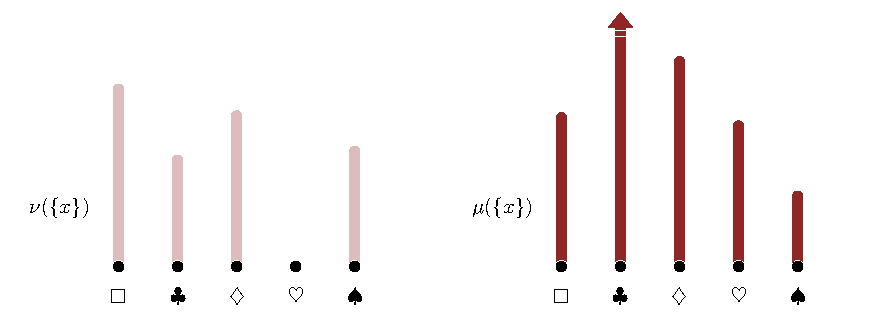
\includegraphics[width=0.9\textwidth,height=\textheight]{figures/scaling_mass_functions/scaling_mass_functions.pdf}

}

\caption{\label{fig-scaling-mass-functions}The atomic allocations from
one discrete measure cannot be consistently scaled into the atomic
allocations of any other discrete measure. For example there is no real
number that will scale the finite allocation \(\nu(\{ \clubsuit \})\)
into the infinite allocation \(\mu(\{ \clubsuit \})\). Similarly there
is no real number that will consistently scale the zero allocation
\(\nu(\{ \heartsuit \})\) into the non-zero allocation
\(\mu(\{ \heartsuit \})\). Consistent scaling requires that all of the
atomic allocations are finite and that the atomic allocations of the
initial measure \(\nu\) are zero only when the atomic allocations of the
second measure \(\mu\) are also zero.}

\end{figure}

Similarly we can translate \(\nu\) integrals into \(\mu\) integrals only
when the atomic allocations are finite and \[
\mathsf{z}_{\mu} \subseteq \mathsf{z}_{\nu}.
\] Importantly these two conditions are not symmetric: we can translate
back \emph{and} forth between \(\mu\) and \(\nu\) integrals only when
the null allocations are the same, \[
\mathsf{z}_{\mu} = \mathsf{z}_{\nu}.
\]

\hypertarget{general-spaces}{%
\subsection{General Spaces}\label{general-spaces}}

Translating integrals between more general measure spaces requires a
generalization of the atomic allocation conditions that we derived in
the previous section to arbitrary allocations. Unsurprisingly this
generalization will take a bit more care.

In this section we'll assume a measurable space \((X, \mathcal{X})\) and
two measures \(\mu : \mathcal{X} \rightarrow [0, \infty]\) and
\(\nu : \mathcal{X} \rightarrow [0, \infty]\).

\hypertarget{sigma-finite-measures}{%
\subsubsection{\texorpdfstring{{\(\sigma\)}-Finite
Measures}{\textbackslash sigma-Finite Measures}}\label{sigma-finite-measures}}

Avoiding infinite atomic allocations is necessary on general measure
spaces, but it is not sufficient for translating integrals from one
measure to another. To avoid any mathematical inconsistencies we also
need to limit exactly which subsets can be allocated infinite measure.
Intuitively we need to avoid infinite ``local'' allocations even if the
total measure is infinite.

To formalize this intuition we will first need to divide the ambient
space into disjoint subsets that probe that local structure. A
\textbf{partition} of \(X\) is any collection of subsets, \[
\mathcal{P}
= \{ \mathsf{x}_{1}, \ldots, \mathsf{x}_{i}, \ldots \},
\] that are non-empty, \[
\mathsf{x}_{i} \ne \emptyset,
\] mutually disjoint, \[
\mathsf{x}_{i} \cap \mathsf{x}_{i' \ne i} = \emptyset,
\] and cover the entire space, \[
\cup_{i} \mathsf{x}_{i} = X.
\] When working with measures we need to restrict attention to
\textbf{measurable partitions}, which contain only measurable subsets,
and \textbf{countable partitions}, which contain only a countable number
of subsets.

For example the full set \(X\) by itself always defines a partition, as
does the collection of atomic subsets. The collection of atomic subsets,
however, will not always define a countable partition. On ordered metric
spaces, such as real lines, measurable and countable partitions built up
from intervals of constant length are particularly natural.

In general we can partition a measurable space in many different ways;
some partitions will divide the space up into smaller subsets than
others. If every subset in one measurable partition \(\mathcal{P}\) is
encapsulated by a subset in another measurable partition
\(\mathcal{P}'\), so that we can construct \(\mathcal{P}\) by breaking
up the subsets in \(\mathcal{P}'\), then we say that \(\mathcal{P}\) is
a \emph{refinement} of \(\mathcal{P}'\). The more refined a measurable
partition is the more sensitively it will be able to probe the ``local''
structure of a measure (Figure~\ref{fig-partition-refinements}).

\begin{figure}

{\centering 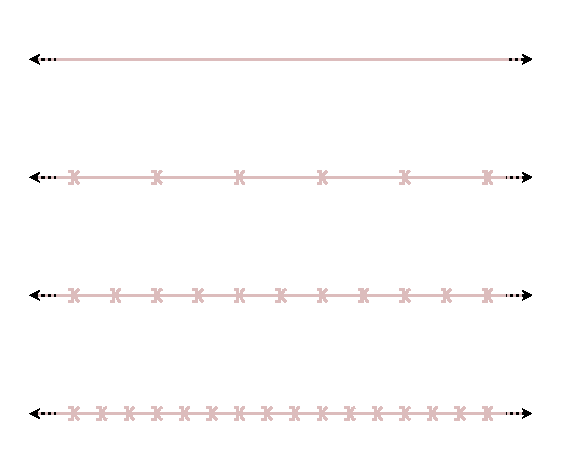
\includegraphics[width=0.5\textwidth,height=\textheight]{figures/partition_refinements/partition_refinements.pdf}

}

\caption{\label{fig-partition-refinements}Every real line can be
partitioned into half-open intervals of constant length. The narrower
the intervals the more refined the partition will be, and the more
sensitive the individual subsets will to the local structure of a
measure. Decomposing a real line all the way into atomic elements
results in a valid partition, but not a countable partition.}

\end{figure}

Every partition is a refinement of the partition defined by the full set
\(X\) alone, making it the crudest possible partition. At the same time
because the partition defined by the atomic subsets is a refinement of
every other partition it is finest possible partition. Both of these
extreme partitions are typically measurable, but the atomic partition
will be countable on only countable spaces.

When the total measure is infinite then the allocations to the subsets
in a crude measurable partition might also be infinite. If we break up
those subsets into finer and finer pieces, however, then the infinite
allocations might spread out into finite allocations. When we can
construct a fine enough measurable partition such that \emph{all} of the
subset allocations are finite we will always able to avoid infinity
entirely by working with small enough subsets. Moreover if that fine
enough measurable partition is also countable then we will always be
able to aggregate those smaller-subset allocations into any general
allocation.

More formally a measure \(\mu\) is \textbf{\(\sigma\)-finite} if we can
construct \emph{at least one} measurable and countable partition where
each subset is allocated only a finite measure, \[
\mu(\mathsf{x}_{i}) < \infty
\] for all \(\mathsf{x}_{i} \in \mathcal{P}\).

Every finite measure, including every probability distribution, is
\(\sigma\)-finite because we can always take the trivial partition
\(\mathcal{P} = \{ X \}\) with \[
\mu(X) < \infty.
\]

On the other hand only exceptional infinite measures are also
\(\sigma\)-finite. For example we can show that every counting measure
\(\chi\) is \(\sigma\)-finite by employing a countable atomic partition,
\[
\mathcal{P} = \{ \{ x \} \mid x \in X \},
\] with \[
\chi( \mathsf{x} ) = 1 < \infty
\] for all \(\mathsf{x} \in \mathcal{P}\). Similarly we can show that
every Lebesgue measure \(\lambda\) is \(\sigma\)-finite by partitioning
a real line into intervals of constant length \(L\), \[
\mathcal{P} =
\{ ( L \cdot n, L \cdot (n + 1) ] \mid n \in \ldots, -1, 0, 1, \ldots \},
\] with \[
\lambda( \mathsf{x} ) = L < \infty
\] for all \(\mathsf{x} \in \mathcal{P}\). Even though the local
interval allocations are finite individually they aggregate into the
infinite total Lebesgue measure.

One immediate obstruction to \(\sigma\)-finiteness is the allocation of
infinite measure to a single atomic subset. Because we can't break an
atomic subset down any further there's no way to diffuse that infinite
allocation into something finite. Fortunately this extreme behavior
rarely if ever show up in practical applications.

Every application that we will consider in this book will only ever use
\(\sigma\)-finite measures.

\hypertarget{absolute-continuity}{%
\subsubsection{Absolute Continuity}\label{absolute-continuity}}

On finite spaces the compatibility between two measures was determined
by the overlap of the null atomic subsets. On more general spaces we
have to consider the overlap of \emph{all} null subsets.

When every \(\nu\)-null subset is a \(\mu\)-null subset, \[
\mathcal{X}_{\nu = 0} \subseteq \mathcal{X}_{\mu = 0}
\] we can say that \(\mu\) is \textbf{absolutely continuous} with
respect to \(\nu\) and write \[
\mu \ll \nu.
\] Equivalently we can say that \(\nu\) \textbf{dominates} \(\mu\).

Because absolute continuity is defined by the null subsets, and not the
precise allocations across non-null subsets, understanding of the null
subsets alone allows us to characterize how compatible two measures are
with each other. In particular when a collection of measures all share
the \emph{same} null subsets then each measure will be absolutely
continuous with respect to every other measure, regardless of their
idiosyncratic behaviors.

For example on a discrete space every measure with non-zero atomic
allocations is absolutely continuous with respect to every other measure
with non-zero atomic allocations. Moreover Lebesgue meaures defined with
respect to different metrics are always absolutely continuous with each
other.

\hypertarget{radon-nikodym-derivatives}{%
\subsubsection{Radon-Nikodym
Derivatives}\label{radon-nikodym-derivatives}}

With \(\sigma\)-finiteness and absolute continuity established we are
now ready to define the most general circumstances under which we can
translate integrals from one measure to another.

If \(\mu\) and \(\nu\) are two \(\sigma\)-finite measures on
\((X, \mathcal{X})\) and \(\mu\) is absolutely continuous with respect
to \(\nu\), \[
\mu \ll \nu,
\] then at least one \(\mathcal{X}\)-measurable, positive real-valued
function \[
\frac{ \mathrm{d} \mu }{ \mathrm{d} \nu } : X \rightarrow \mathbb{R}^{+}
\] exists such that \[
\mathbb{I}_{\mu}[f] =
\mathbb{I}_{\nu} \left[
\frac{ \mathrm{d} \mu }{ \mathrm{d} \nu } \cdot f
\right]
\] for \emph{every} \(\mathcal{X}\)-measurable, \(\mu\)-integrable,
real-valued function \(f : X \rightarrow \mathbb{R}\).

Any such function \(\mathrm{d} \mu / \mathrm{d} \nu\) that translates
\(\mu\) integrals into \(\nu\) integrals is known as a
\textbf{Radon-Nikodym derivative} of \(\mu\) with respect to \(\nu\). In
this case \(\mu\) is denoted the \textbf{target} measure and \(\nu\) is
denoted the \textbf{reference} measure.

Because Radon-Nikodym derivatives are defined by measure-informed
integrals they are not, in general, unique. Modifying the outputs of a
Radon-Nikodym derivative on a \(\nu\)-null subset of inputs results in
the same \(\nu\) integrals, and hence another valid Radon-Nikodym
derivative. In practice we can usually restrict our consideration to
Radon-Nikodym derivatives that also happen to be continuous or even
smooth. These \emph{structured} Radon-Nikodym derivatives are typically
unique for each \(\mu\) and \(\nu\), and we don't lose any generality by
ignoring the others provided that we never try to interpret these
functions outside of the shadow of an integral!

For example the unit function \begin{alignat*}{6}
u :\; & X & &\rightarrow& \; & \mathbb{R}^{+} &
\\
& x & &\mapsto& & 1 &
\end{alignat*} is one possible Radon-Nikodym derivative for any measure
with respect to itself, \[
\frac{ \mathrm{d} \nu }{ \mathrm{d} \nu }
\overset{\nu}{=}
u.
\] At the same time any function that deviates from the unit function
only on \(\nu\)-null subsets is also a valid Radon-Nikodym derivative
for \(\nu\) with respect to itself. If \(X = \mathbb{R}\), however, then
the unit function is the only continuous Radon-Nikodym derivative.

Using the local scaling notation that we introduced in
\href{https://betanalpha.github.io/assets/chapters_html/expectation_values.html}{Chapter
5} we can also express the relationship between two compatible measures
and the Radon-Nikodym derivative that links them together as \[
\mu = \frac{ \mathrm{d} \mu }{ \mathrm{d} \nu } \cdot \nu.
\] Again this is just shorthand for the integral relationships \[
\mathbb{I}_{\mu}[f] =
\mathbb{I}_{\nu} \left[
\frac{ \mathrm{d} \mu }{ \mathrm{d} \nu } \cdot f
\right].
\]

\hypertarget{interpreting-radon-nikodym-derivatives}{%
\subsubsection{Interpreting Radon-Nikodym
Derivatives}\label{interpreting-radon-nikodym-derivatives}}

One way to build intuition for Radon-Nikodym derivatives is to consider
the integral of indicator functions. For any measurable subset
\(\mathsf{x} \in \mathcal{X}\) we have \begin{align*}
\mu( \mathsf{x} )
&=
\mathbb{I}_{\mu} [ I_{\mathsf{x}} ]
\\
&=
\mathbb{I}_{\nu} \left[
\frac{ \mathrm{d} \mu }{ \mathrm{d} \nu } \cdot I_{\mathsf{x}} \right].
\end{align*} If \[
\mathrm{d} \mu / \mathrm{d} \nu(x) > 1
\] for \emph{almost all} points \(x \in \mathsf{x}\) -- remember that we
always have to excuse deviant behavior over the null subsets of \(\nu\)
-- then we will also have \[
\frac{ \mathrm{d} \mu }{ \mathrm{d} \nu }(x) \cdot I_{\mathsf{x}}(x)
> I_{\mathsf{x}}(x)
\] for almost all \(x \in X\). This implies that \begin{align*}
\mu( \mathsf{x} )
&=
\mathbb{I}_{\nu} \left[
\frac{ \mathrm{d} \mu }{ \mathrm{d} \nu } \cdot I_{\mathsf{x}} \right]
\\
&>
\mathbb{I}_{\nu} \left[ I_{\mathsf{x}} \right]
\\
&>
\nu(\mathsf{x}),
\end{align*} or \[
\mu( \mathsf{x} ) > \nu( \mathsf{x} ).
\]

In other words if \[
\mathrm{d} \mu / \mathrm{d} \nu(x) > 1
\] across some subset of the ambient space then \(\mu\) will allocate
\emph{more} measure there than \(\nu\). The larger the Radon-Nikodym
derivative is the more excessive the \(\mu\) allocation will be.
Similarly if \[
\mathrm{d} \mu / \mathrm{d} \nu(x) < 1
\] across some subset then \(\mu\) will allocate \emph{less} measure
there than \(\nu\). At the extreme any measurable collection of points
with \[
\mathrm{d} \mu / \mathrm{d} \nu(x) \overset{\nu}{=} 0
\] always defines a \(\mu\)-null subset. In between if \[
\mathrm{d} \mu / \mathrm{d} \nu(x) \overset{\nu}{=} 1
\] across a subset then \(\mu\) and \(\nu\) will allocate the
\emph{same} measure to that subset.

Consequently we can interpret a Radon-Nikodym derivative as quantifying
how the allocations of \(\mu\) are \emph{locally} enhanced or suppressed
relative to the allocations of \(\nu\). By integrating indicator
functions we aggregate these local warpings into non-local changes in
the subset allocations.

A common physical analogy is to interpret the reference measure \(\nu\)
as defining a sense of \emph{volume} across the ambient space. The more
measure \(\nu\) allocates to a given subset the more background volume
is spanned by that subset. If we analogize the measure allocated by
\(\mu\) to a physical \emph{mass} then Radon-Nikodym derivatives become
\textbf{density functions} that quantify how strongly mass concentrates
within any given volume.

Personally I've always found the term ``Radon-Nikodym derivative'' to be
aesthetically pleasing -- it sounds like a term straight out of science
fiction to me -- but this density function analogy is typically much
more accessible. Because of that I will use the term ``density
function'' instead of ``Radon-Nikodym derivative'' as much as possible.

\hypertarget{operator-perspective}{%
\subsubsection{Operator Perspective}\label{operator-perspective}}

Speaking of terminology, why do we call a Radon-Nikodym derivative a
``derivative'' in the first place? It turns out that mathematically
Radon-Nikodym derivatives do satisfy the properties of formal
derivatives, but the theory needed to demonstrate that is pretty
elaborate. In this section we will instead investigate some of the more
superficial similarities between Radon-Nikodym derivative and the
familiar derivatives from calculus.

Recall that in one-dimensional calculus differentiation is an operation
that converts a smooth function \(f: \mathbb{R} \rightarrow \mathbb{R}\)
into a \emph{new} function \[
\frac{ \mathrm{d} f }{ \mathrm{d} x} :
\mathbb{R} \rightarrow \mathbb{R}.
\] This operation is linear, \[
\frac{ \mathrm{d} }{ \mathrm{d} x}
\left( \alpha \, f + \beta \, g \right)
=
  \alpha \, \frac{ \mathrm{d} f }{ \mathrm{d} x}
+ \beta \, \frac{ \mathrm{d} g }{ \mathrm{d} x},
\] and satisfies a chain rule, \[
\frac{ \mathrm{d} (g \circ f)}{ \mathrm{d} x}(x)
=
\frac{ \mathrm{d} g}{ \mathrm{d} y}(f(x))
\frac{ \mathrm{d} f}{ \mathrm{d} x}(x)
\] for any two functions \(f: x \mapsto y\) and \(g: y \mapsto z\).

The output of the derivative function at the point \(x \in \mathbb{R}\),
\[
\frac{ \mathrm{d} f }{ \mathrm{d} x}(x),
\] quantifies how quickly \(f\) changes at that input
(Figure~\ref{fig-differentiation}). If \[
\frac{ \mathrm{d} f }{ \mathrm{d} x}(x) > 0
\] then \(f\) is increasing at \(x\), if \[
\frac{ \mathrm{d} f }{ \mathrm{d} x}(x) < 0
\] then \(f\) is decreasing at \(x\), and if \[
\frac{ \mathrm{d} f }{ \mathrm{d} x}(x) = 0
\] then \(f\) is constant at \(x\).

\begin{figure}

{\centering 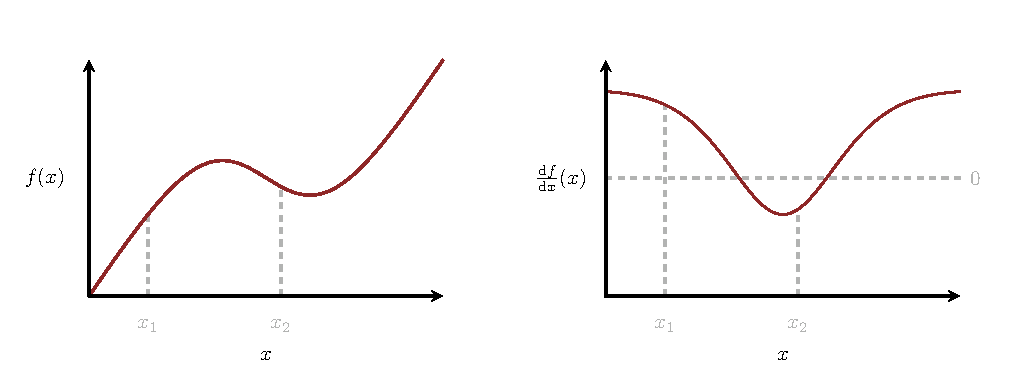
\includegraphics[width=0.9\textwidth,height=\textheight]{figures/differentiation/differentiation.pdf}

}

\caption{\label{fig-differentiation}The derivative
\(\mathrm{d} f / \mathrm{d} x\) of a function \(f\) is itself a function
that quantifies how \(f\) changes at each point \(x \in \mathbb{R}\).
Because \(f\) is increasing at \(x_{1}\) the derivative is positive
there, \(\mathrm{d} f / \mathrm{d} x (x_{1}) > 0\). Similarly because
\(f\) is decreasing at \(x_{2}\) the derivative is negative there. We
can also interpret the derivative as quantifying how much \(f\) changes
\emph{relative} to a constant function. Because
\(\mathrm{d} f / \mathrm{d} x (x_{1}) > 0\) the function \(f\) is
increasing faster than the constant function at \(x_{1}\). At the same
time because \(\mathrm{d} f / \mathrm{d} x (x_{2}) < 0\) the function
\(f\) is increasing more slowly than the constant function at
\(x_{2}\).}

\end{figure}

Equivalently we can interpret a derivative function as quantifying how
much the initial function changes \emph{relative to a constant
function}. If \[
\frac{ \mathrm{d} f }{ \mathrm{d} x}(x) > 0
\] then \(f\) is increasing \emph{faster} than a constant function at
\(x\), if \[
\frac{ \mathrm{d} f }{ \mathrm{d} x}(x) < 0
\] then \(f\) is increasing \emph{slower} than a constant function at
\(x\), and if \[
\frac{ \mathrm{d} f }{ \mathrm{d} x}(x) = 0
\] then \(f\) is increasing \emph{at the same rate} as a constant
function at \(x\). In other words we can interpret the derivative as an
operator that gives an output function that quantifies how much the
input function changes relative to some reference behavior.

Similarly we can interpret Radon-Nikodym derivatives as the output of an
operator that gives output functions that quantify how much an input
measure changes relative to some reference measure. Even more this
operator is linear and satisfies a chain rule.

To formalize this similarity a bit more let's use \(M(X, \mathcal{X})\)
to denote the collection of all measures that we can define over the
measurable space \((X, \mathcal{X})\) and \(C^{+}(X, \mathcal{X}, \mu)\)
to denote the collection of all \(\mathcal{X}\)-measurable functions
from \(X\) to \(\mathbb{R}^{+}\). We can then define
\textbf{Radon-Nikodym differentiation} as a mapping \begin{alignat*}{6}
\frac{ \mathrm{d} }{ \mathrm{d} \nu } :\; & M(X, \mathcal{X}) & &\rightarrow& \;
& C^{+}(X, \mathcal{X}) &
\\
& \mu & &\mapsto& & \frac{ \mathrm{d} \mu }{ \mathrm{d} \nu } &
\end{alignat*} that takes an input measure \(\mu\) to an output function
\[
\frac{ \mathrm{d} \mu }{ \mathrm{d} \nu } : X \rightarrow \mathbb{R}^{+}
\] that captures how \(\mu\) varies relative to \(\nu\).

Admittedly I'm being a bit mathematically sloppy here because
Radon-Nikodym derivatives are defined only up to \(\nu\)-null subsets;
technically this mapping doesn't yield a single function but rather a
collection of all functions that are equal \(\nu\)-almost everywhere. In
order to achieve a unique outptu function we need to introduce
additional constraints, such as continuity or even smoothness. This
sloppy notation, however, does allow us to investigate many of the
useful properties of the operation.

For example Radon-Nikodym differentiation is linear. If we define a
linear combination of measures by the allocations \[
(\alpha \cdot \mu + \beta \cdot \nu)(\mathsf{x})
=
\alpha \cdot \mu(\mathsf{x}) + \beta \cdot \nu(\mathsf{x})
\] then \[
\frac{ \mathrm{d} }{ \mathrm{d} \lambda }
(\alpha \cdot \mu + \beta \cdot \nu)
\overset{\nu}{=}
\alpha \cdot \frac{ \mathrm{d} \mu}{ \mathrm{d} \lambda }
+ \beta \cdot \frac{ \mathrm{d} \nu }{ \mathrm{d} \lambda }
\] whenever \(\mu\) and \(\nu\) are both absolutely continuous with
respect to \(\lambda\), \[
\mathcal{X}_{\lambda = 0} \subseteq
\mathcal{X}_{\mu = 0} \cap \mathcal{X}_{\nu = 0}.
\] Note that to be technically correct, the best kind of correct,
equalities like these hold only up to \(\nu\)-null subsets.

Similarly Radon-Nikodym differentiation satisfies a chain rule. If
\(\mu\) is absolutely continuous with respect to \(\lambda\) and
\(\lambda\) is absolutely continuous with respect to \(\nu\), \[
\mathcal{X}_{\mu = 0}
\subseteq \mathcal{X}_{\lambda = 0}
\subseteq \mathcal{X}_{\nu = 0},
\] then \[
\frac{ \mathrm{d} \mu}{ \mathrm{d} \nu}
\overset{\nu}{=}
\frac{ \mathrm{d} \mu}{ \mathrm{d} \lambda } \cdot
\frac{ \mathrm{d} \lambda}{ \mathrm{d} \nu }.
\] Again we have to be careful to acknowledge that this ``equality''
holds only up to \(\nu\)-null subsets.

The Radon-Nikodym chain rule can be particularly useful in practice when
we're interested in comparing two measures \(\mu\) and \(\nu\) to each
other but a third measure \(\lambda\) is a more convenient reference
measure. For example consider the simplified case where \(\mu\),
\(\nu\), and \(\lambda\) all share the same null subsets, \[
  \mathcal{X}_{\mu = 0}
= \mathcal{X}_{\nu = 0}
= \mathcal{X}_{\lambda = 0}
\equiv \mathcal{X}_{0},
\] and hence are all absolutely continuous with respect to each other.
In this case all of the Radon-Nikodym derivatives between these measures
are almost everywhere non-zero and we can write \begin{align*}
1
&\overset{\nu}{=}
\frac{ \mathrm{d} \nu}{ \mathrm{d} \nu}(x)
\\
1
&\overset{\nu}{=}
\frac{ \mathrm{d} \nu}{ \mathrm{d} \lambda }(x) \cdot
\frac{ \mathrm{d} \lambda}{ \mathrm{d} \nu }(x)
\end{align*} or \[
\frac{ \mathrm{d} \lambda}{ \mathrm{d} \nu }(x)
\overset{\nu}{=}
\frac{1}{ \frac{ \mathrm{d} \nu}{ \mathrm{d} \lambda }(x) }
\] up to the common null subsets.

Consequently we can write the Radon-Nikodym derivative between \(\mu\)
and \(\nu\) as a ratio of the Radon-Nikodym derivatives with respect to
\(\lambda\), \begin{align*}
\frac{ \mathrm{d} \mu}{ \mathrm{d} \nu}(x)
&\overset{\nu}{=}
\frac{ \mathrm{d} \mu}{ \mathrm{d} \lambda }(x) \cdot
\frac{ \mathrm{d} \lambda}{ \mathrm{d} \nu }(x)
\\
&\overset{\nu}{=}
\frac{ \mathrm{d} \mu}{ \mathrm{d} \lambda }(x) \cdot
\frac{1}{ \frac{ \mathrm{d} \nu}{ \mathrm{d} \lambda }(x) }
\\
&\overset{\nu}{=}
\frac{ \frac{ \mathrm{d} \mu}{ \mathrm{d} \lambda }(x) }
{ \frac{ \mathrm{d} \nu}{ \mathrm{d} \lambda }(x) }.
\end{align*} In this way we can directly compare the behaviors of
\(\mu\) and \(\nu\) to each other using only the more convenient
Radon-Nikodym derivatives.

\hypertarget{specifying-probability-distributions-with-density-functions}{%
\section{Specifying Probability Distributions With Density
Functions}\label{specifying-probability-distributions-with-density-functions}}

The initial use case for density functions, née Radon-Nikodym
derivatives, requires the selection of a target measure and a reference
measure \(\nu\). In this setting we can translate implicit integrals
with respect to the target measure to explicit integrals with respect to
the reference measure, \[
\mathbb{I}_{\mu}[f] =
\mathbb{I}_{\nu}
\left[ \frac{ \mathrm{d} \pi}{ \mathrm{d} \nu } \cdot f \right].
\]

This construction, however, can also be reversed. Given a reference
measure, any measurable, positive-real valued function implicitly
defines a target measure without having to directly specify any subset
allocations.

Consider, for example, a measurable space \((X, \mathcal{X})\) and a
convenient, \(\sigma\)-finite measure \(\nu\). Every non-negative,
\(\mathcal{X}\)-measurable function \(m : X \rightarrow R^{+}\)
implicitly defines a measure \(\mu\) with the measure-informed integrals
\[
\mathbb{I}_{\mu}[f] = \mathbb{I}_{\nu} \left[ m \cdot f \right].
\]

The \textbf{normalization} of a density function is defined by its
integral with respect to the reference measure,
\(\mathbb{I}_{\nu}[ m ]\). If \[
\mathbb{I}_{\nu}[ m ] = 1
\] then the total induced measure becomes \begin{align*}
\mu(X)
&=
\mathbb{I}_{\mu}[I_{X}]
\\
&=
\mathbb{I}_{\nu} [ m \cdot I_{X} ]
\\
&=
\mathbb{I}_{\nu} [ m ]
\\
&=
1.
\end{align*} Consequently a properly normalized density function defines
not just a measure but a probability distribution.

In other words every non-negative, \(\mathcal{X}\)-measurable function
\(p : X \rightarrow R^{+}\) with unit normalization,
\(\mathbb{I}_{\nu} [ p ] = 1\), implicitly defines a probability
distribution \(\pi\) with the expectation values \[
\mathbb{E}_{\pi}[f] = \mathbb{I}_{\nu} \left[ p \cdot f \right].
\] Because we will be working with mostly probability distributions in
practice, we will be working with mostly these probability density
functions.

Note that, while the probabilities given by evaluating a probability
distribution can take only real values between zero and one, the
probability densities given by evaluating a probability density function
can take \emph{any} non-negative real value. Probability densities and
probabilities are distinct and should not be confused with each other!

In practice working with point-wise functions is much easier than
working with subset-wise functions. For example when the ambient space
is low-dimensional we can visualize point-wise functional behavior
directly, allowing density functions to not define probability
distributions but also communicate their behaviors. We'll explore this
latter feature in the context of Lebesgue reference measures in
\href{@sec:visualizing}{Section 4.3}.

This is not to say that probability density functions are not without
their limitations. In particular probability density functions are
defined only relative to the given reference measure. If the reference
measure is at all ambiguous then a density function will not completely
determine a probability distribution! At the same time if the reference
measure every changes then probability density functions will also have
to change if we want them to represent the same probability
distributions.

We will use probability density functions to define relevant probability
distributions almost exclusively in this book. In the cases where we
start with a probability distribution \(\pi\) and reference measure
\(\nu\) then I will use the notation \[
\frac{ \mathrm{d} \pi}{ \mathrm{d} \nu}
\] for the corresponding probability density function. This notation is
both compact and explicit, display all of the information needed to put
the density function into context.

Most of the time, however, we don't start with an explicit probability
distribution but rather a reference measure \(\nu\) and a properly
normalized function \(p : X \rightarrow \mathbb{R}^{+}\) to implicitly
define a probability distribution, \[
\pi = p \cdot \nu,
\] or, equivalently, \[
\mathbb{E}_{\pi}[f] = \mathbb{I}_{\nu}[p \cdot f].
\] In these more common cases I will use Roman letters to denote
probability density functions. Whenever possible I will also match the
Roman letter used to denote a probability density function and the Greek
letter used to denote the induced probability distribution.

The only limitation of this latter notational convention is that it
doesn't communicate the underlying reference measure. Because of this it
is not difficult to lose track of that reference measure, especially
when multiple reference measures might be relevant in a given
application.

Unfortunately this convention has also become standard in many fields,
and it is nearly impossible to avoid in practice. To avoid any confusion
when we encounter a probability density function
\(p : X \rightarrow \mathbb{R}^{+}\) we have to take care to consider
what the accompanying reference measure is.

\hypertarget{probability-density-functions-on-discrete-measure-spaces}{%
\section{Probability Density Functions on Discrete Measure
Spaces}\label{probability-density-functions-on-discrete-measure-spaces}}

Now that we have defined probability density functions in full
generality we can study how they're used in the kinds of spaces that
often arise in practical applications. We'll begin by looking at
probability density functions on discrete measure spaces.

\hypertarget{probability-mass-functions}{%
\subsection{Probability Mass
Functions}\label{probability-mass-functions}}

On discrete measurable spaces \((X, 2^{X})\) we can always construct a
uniform counting measure that allocates a unit measure to each atomic
subset, \[
\chi( \{ x \} ) = 1.
\] Because a counting measure doesn't have any null subsets it dominates
\emph{every} measure that we could define on \((X, 2^{X})\), making it a
natural reference measure for any discrete probability distribution.
Moreover the lack of null subsets also means that density functions will
always be unique.

Following the steps we worked through in
\href{@sec:finite_densities}{Section 1.1} we can derive an explicit
result for the probability density function defined by any probability
distribution \(\pi\) with respect to a counting measure. Translating an
expectation value to an integral informed by the counting measure gives
\begin{align*}
\mathbb{E}_{\pi}[f]
&=
\sum_{x \in X}
\pi( \{ x \} ) \cdot f(x)
\\
&=
\sum_{x \in X}
1 \cdot \pi( \{ x \} ) \cdot f(x)
\\
&=
\sum_{x \in X}
\chi( \{ x \} ) \cdot \pi( \{ x \} ) \cdot f(x)
\\
&=
\sum_{x \in X}
\chi( \{ x \} ) \cdot \left( \pi( \{ x \} ) \cdot f(x) \right)
\\
&=
\mathbb{I}_{\chi} [ \pi \cdot f ],
\end{align*} where \(\pi\) in the last term denotes a function maps each
element of \(X\) to its atomic allocation, \begin{alignat*}{6}
\pi :\; & X & &\rightarrow& \; & [0, \infty] &
\\
& x & &\mapsto& & \pi( \{ x \} ) &.
\end{alignat*}

In other words the density of any probability distribution with respect
to the counting measure is just the corresponding probability mass
function, \[
\frac{ \mathrm{d} \pi }{ \mathrm{d} \chi }(x) = \pi(x)!
\] Because of this association probability mass functions are also
sometimes referred to as discrete probability density functions.

Identifying probability mass functions with Radon-Nikodym derivatives
not only formalizes all of the more heuristic results that we've
developed on countable spaces but also places them within the context of
the more general probability theory. For example when we use the atomic
allocations specified by a probability mass function to compute
expectation values we're implicitly integrating with respect to a
counting measure. Similarly when we visualize a probability distribution
by plotting the atomic allocations we're communicating how much the
probability distribution warps the uniform allocations defined by the
counting measure.

\hypertarget{the-poisson-family-of-probability-mass-functions}{%
\subsection{The Poisson Family of Probability Mass
Functions}\label{the-poisson-family-of-probability-mass-functions}}

To demonstrate the use of probability density functions on countable
spaces let's consider the positive integers,
\((\mathbb{N}, 2^{\mathbb{N}})\). Assuming the counting measure we can
specify an entire \emph{family} of probability distributions with the
parametrized probability density function (Figure~\ref{fig-poisson}) \[
\mathrm{Poisson}(n; \lambda) = \frac{ \lambda^{n} e^{-\lambda} }{ n! },
\] where \(\lambda \in \mathbb{R}^{+}\).

\begin{figure}

\begin{minipage}[t]{0.01\linewidth}

{\centering 

~

}

\end{minipage}%
%
\begin{minipage}[t]{0.33\linewidth}

{\centering 

\raisebox{-\height}{

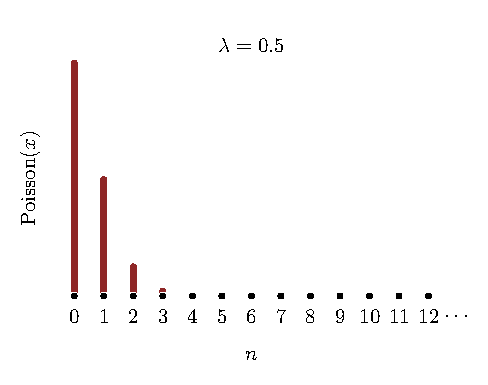
\includegraphics{figures/poisson/mass_functions/1/1.pdf}

}

}

\subcaption{\label{fig-poisson1}}
\end{minipage}%
%
\begin{minipage}[t]{0.33\linewidth}

{\centering 

\raisebox{-\height}{

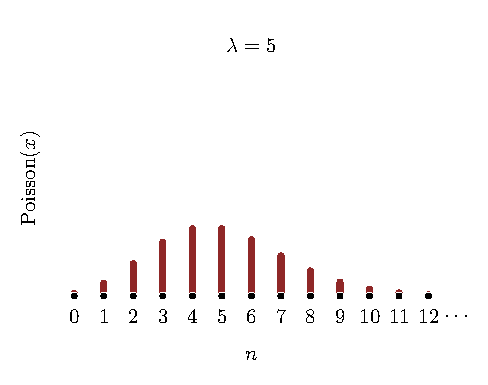
\includegraphics{figures/poisson/mass_functions/2/2.pdf}

}

}

\subcaption{\label{fig-poisson2}}
\end{minipage}%
%
\begin{minipage}[t]{0.33\linewidth}

{\centering 

\raisebox{-\height}{

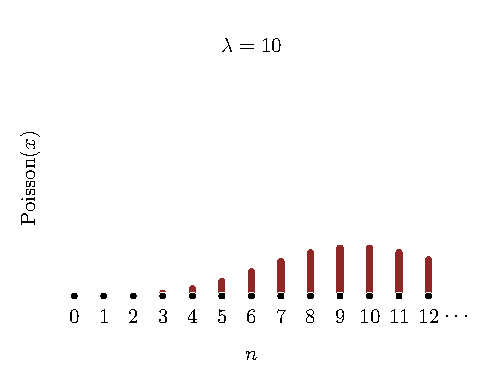
\includegraphics{figures/poisson/mass_functions/3/3.pdf}

}

}

\subcaption{\label{fig-poisson3}}
\end{minipage}%
%
\begin{minipage}[t]{0.01\linewidth}

{\centering 

~

}

\end{minipage}%

\caption{\label{fig-poisson}For each value of the parameter \(\lambda\)
the Poisson family \(\mathrm{Poisson}(n; \lambda)\) defines a discrete
probability density function, and hence a probability distribution in
the context of a reference counting measure. As \(\lambda\) increases
from (a) to (c) the probability distributions concentrate are larger
integers.}

\end{figure}

This family of probability mass functions, as well as the family of
probability distributions they implicitly define, is known as the
\textbf{Poisson} family. If we fix \(\lambda\) then
\(\mathrm{Poisson}(n; \lambda)\) denotes a Poisson probability mass
function, and implicitly Poisson distribution.

Expectation values with respect to a Poisson distribution are given by
explicit summations, \begin{align*}
\mathbb{E}_{\mathrm{Poisson}}[ f ; \lambda ]
&=
\mathbb{I}_{\chi}[ \mathrm{Poisson}( ; \lambda) \cdot f ]
\\
&=
\sum_{n = 0}^{\infty} \mathrm{Poisson}(n; \lambda) \, f(n).
\end{align*} The sums for many common expectands can actually be worked
out in closed form. I've isolated those calculations in the
\href{@sec:appendix}{Appendix} and will simply state some of the more
important results here.

For example the normalization of each Poisson probability mass function
is unity, \begin{align*}
\mathrm{Poisson}(X; \lambda)
&= \mathbb{E}_{\mathrm{Poisson}}[ I_{X}; \lambda ]
\\
&= \mathbb{I}_{\chi}[ \mathrm{Poisson}( ; \lambda) \cdot I_{X} ]
\\
&= \sum_{n = 0}^{\infty} \mathrm{Poisson}(n; \lambda) \cdot 1
\\
&= 1,
\end{align*} as required.

Similarly the mean for each Poisson probability distribution is given by
\begin{align*}
\mathbb{M}(\lambda)
&=
\mathbb{E}_{\mathrm{Poisson}} [ \iota ; \lambda ]
\\
&=
\mathbb{I}_{\chi} [ \mathrm{Poisson}( ; \lambda) \cdot \iota ]
\\
&= \sum_{n = 0}^{\infty} \mathrm{Poisson}(n; \lambda) \cdot \iota(n)
\\
&= \lambda.
\end{align*} Consequently the parameter \(\lambda\) moderates the
centrality of probability distributions defined by each Poisson mass
functions (Figure~\ref{fig-poisson-mean}).

\begin{figure}

{\centering 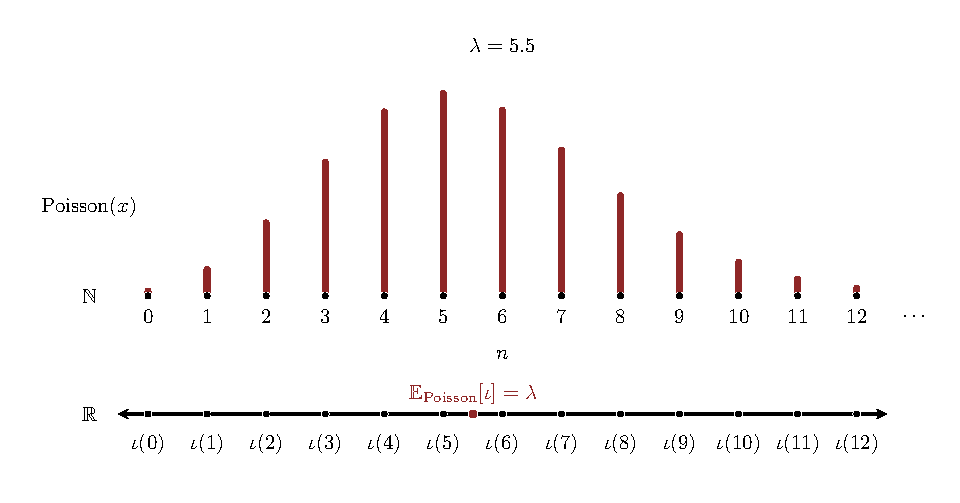
\includegraphics[width=0.8\textwidth,height=\textheight]{figures/poisson/mean/mean.pdf}

}

\caption{\label{fig-poisson-mean}The positive real-valued parameter
\(\lambda\) determines the centrality of each Poisson probability mass
function, and hence each Poisson probability distribution. Recall that
even though the ambient space is discrete the mean will in general take
on real values.}

\end{figure}

A slightly longer calculation shows that the variance of each Poisson
distribution is also equal to \(\lambda\). As we increase the parameter
\(\lambda\) the individual Poisson distributions not only shift to
larger values but also become more diffuse.

The Poisson cumulative distribution functions \[
\Pi(n)
= \mathrm{Poisson}([0, n]; \lambda)
= \sum_{n' = 0}^{n} \mathrm{Poisson}(n'; \lambda)
\] can also be evaluated in closed form, \[
\Pi(n) = \frac{ \Gamma(n + 1, \lambda) }{ \Gamma(n + 1) },
\] where \(\Gamma(x, y)\) is the \textbf{incomplete Gamma function} and
\(\Gamma(x)\) is the \textbf{gamma function}. Conveniently these two
functions, if not the Poisson cumulative distribution function itself,
are implemented in most programming languages, making them
straightforward to use in practice.

These cumulative distribution functions give us two ways to evaluate
interval probabilities (Figure~\ref{fig-poisson-interval-prob}). On one
hand we can brute force an interval probability with direct summation,
\[
\mathrm{Poisson}( \, (n_{1}, n_{2}] \, ; \lambda)
=
\sum_{n' = n_{1} + 1}^{n_{2}} \mathrm{Poisson}(n'; \lambda).
\] On the other hand we can evaluate the cumulative distribution
function at each boundary and subtract, \[
\mathrm{Poisson}( \, (n_{1}, n_{2}] \, ; \lambda) f
=
\Pi_{\mathrm{Poisson}}(n_{2}) - \Pi_{\mathrm{Poisson}}(n_{1}).
\]

\begin{figure}

\begin{minipage}[t]{0.05\linewidth}

{\centering 

~

}

\end{minipage}%
%
\begin{minipage}[t]{0.45\linewidth}

{\centering 

\raisebox{-\height}{

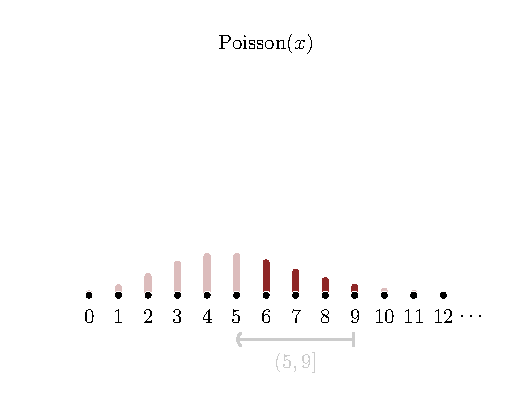
\includegraphics{figures/poisson/interval_prob/sum/sum.pdf}

}

}

\subcaption{\label{fig-poisson-sum}}
\end{minipage}%
%
\begin{minipage}[t]{0.45\linewidth}

{\centering 

\raisebox{-\height}{

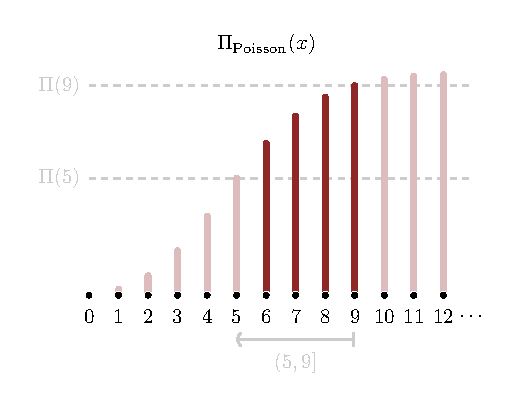
\includegraphics{figures/poisson/interval_prob/difference/difference.pdf}

}

}

\subcaption{\label{fig-poisson-diff}}
\end{minipage}%
%
\begin{minipage}[t]{0.05\linewidth}

{\centering 

~

}

\end{minipage}%

\caption{\label{fig-poisson-interval-prob}The interval probabilities
allocated by Poisson probability distributions can be computed by (a)
exhaustively summing over all of the points in an interval of (b)
substracting the output of the cumulative distribution function at the
interval boundaries.}

\end{figure}

\hypertarget{probability-density-functions-on-real-spaces}{%
\section{Probability Density Functions on Real
Spaces}\label{probability-density-functions-on-real-spaces}}

Having explored discrete measure spaces let's consider our prototypical
uncountable spaces, the spaces of real numbers. On these spaces we don't
have heuristics on which we can fall back, and the full machinery of
Radon-Nikodym derivatives is needed to ensure consistent results. On
these spaces the Lebesgue measure serves as a natural reference measure
and most expectation values reduce not to summations but rather classic
integrals.

\hypertarget{lebesgue-probability-density-functions}{%
\subsection{Lebesgue Probability Density
Functions}\label{lebesgue-probability-density-functions}}

The metric structure of a real space makes Lebesgue measures
particularly useful. In particular because Lebesgue measures are
\(\sigma\)-finite they serve as immediate candidates for reference
measures.

The only remaining obstruction to the construction of probability
density functions is absolute continuity. For practical considerations
the most important Lebesgue null subsets are the subsets consisting of
only a countable number of points; any probability distribution that is
absolutely continuous with respect to the Lebesgue measure must also
allocate zero probability to atomic subsets and their countable unions.
In theory there are other, more abstract, null subsets that need to be
accommodated but the atomic subsets are the most practically relevant.

Given a particular \(D\)-dimensional real space, that is a particular
rigid real space or particular parameterization of a flexible real
space, and a compatible a compatible probability distribution \(\pi\) we
can define a Lebesgue probability density function \[
\frac{ \mathrm{d} \pi \hphantom{ {}^{D} } }{ \mathrm{d} \lambda^{D} } :
\mathbb{R}^{D} \rightarrow \mathbb{R}^{+}.
\]

Alternatively any measurable, positive real-valued function \[
p : \mathbb{R}^{D} \rightarrow \mathbb{R}^{+}
\] that is appropriately normalized, \[
\mathbb{I}_{\lambda^{D}}[ p ]
= \int \mathrm{d}^{D} x \, p(x_{1}, \ldots, x_{d}, \ldots, x_{D})
= 1,
\] will implicitly specify a probability distribution. By construction
these engineered probability distributions will be absolutely continuous
with respect to the defining Lebesgue measure, allocating zero
probability to every atomic subset. In practice almost every probability
distribution over real spaces that we will encounter in applied problems
will be built up by scaling the Lebesgue measure in this way.

Given a one-dimensional Lebesgue probability density function we can
compute the probability allocated to any interval subset with an
appropriately bounded integral, \begin{align*}
\pi( \, [ x_{1}, x_{2} ] \, )
&=
\mathbb{E}_{\pi} \left[ I_{[ x_{1}, x_{2} ]} \right]
\\
&=
\mathbb{I}_{\lambda} \left[
\frac{ \mathrm{d} \pi }{ \mathrm{d} \lambda} \cdot I_{[ x_{1}, x_{2} ]}
\right]
\\
&=
\int_{-\infty}^{+\infty} \mathrm{d} x \,
\frac{ \mathrm{d} \pi }{ \mathrm{d} \lambda}(x) \cdot I_{[ x_{1}, x_{2} ]}(x)
\\
&=
\int_{x_{1}}^{x_{2}} \mathrm{d} x \,
\frac{ \mathrm{d} \pi }{ \mathrm{d} \lambda}(x).
\end{align*} In other words interval probabilities are equal to the
\emph{area} under the curve defined by the probability density function
(Figure~\ref{fig-interval-probs}). For higher-dimensional real spaces
subset probabilities become volumes under the surfaces defined by the
higher-dimensional probability density functions.

\begin{figure}

\begin{minipage}[t]{0.05\linewidth}

{\centering 

~

}

\end{minipage}%
%
\begin{minipage}[t]{0.45\linewidth}

{\centering 

\raisebox{-\height}{

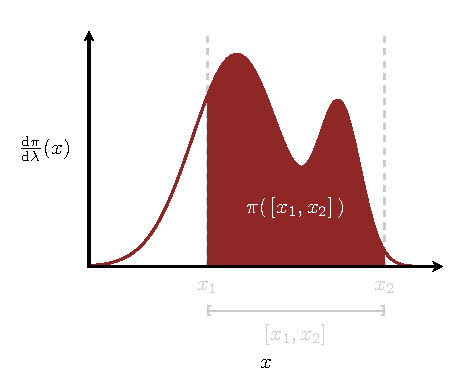
\includegraphics{figures/subset_probabilities/area_under_curve/area_under_curve.pdf}

}

}

\subcaption{\label{fig-area}}
\end{minipage}%
%
\begin{minipage}[t]{0.45\linewidth}

{\centering 

\raisebox{-\height}{

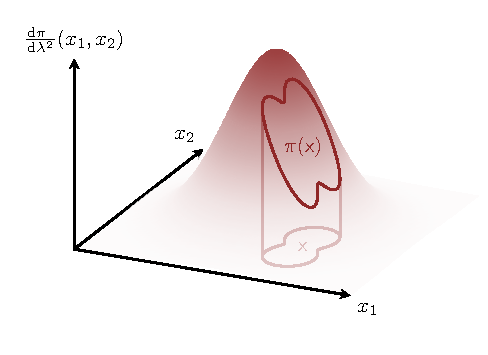
\includegraphics{figures/subset_probabilities/volume_under_curve/volume_under_curve.pdf}

}

}

\subcaption{\label{fig-volume}}
\end{minipage}%
%
\begin{minipage}[t]{0.05\linewidth}

{\centering 

~

}

\end{minipage}%

\caption{\label{fig-interval-probs}Subset probabilities are derived from
Lebesgue probability density functions through classic integration. (a)
One-dimensional interval probabilities are given by the area under the
curve defined by a one-dimensional Lebesgue probability density
function. (b) In higher-dimensions we have to compute the volume under
the surface defined by a Lebesgue probability density function.}

\end{figure}

When working with Lebesgue probability density functions in practice we
have to be \emph{very} careful to account for \emph{which} Lebesgue
measure we're using at any given time. Different real spaces, or
different parameterizations of a single flexible real space, will in
general feature different metrics which then give rise to different
Lebesgue measures.

Because of this a fixed Lebesgue probability density function will
define \emph{different} probability distributions on different real
spaces. Equivalently in order to represent a fixed target probability
distribution \(\pi\) we need to use \emph{different} Lebesgue
probability density functions on every individual real space. Either way
to avoid any ambiguity we need to clearly communicate which Lebesgue
measure we're assuming.

In the next chapter we'll learn how to transform measures from one space
to another. This will allow us to relate the Lebesgue measures, and the
corresponding Lebesgue probability density functions, from one real
space to another, or equivalently from one parameterization of a
flexible real space to another.

\hypertarget{abusing-the-equals-sign}{%
\subsection{Abusing The Equals Sign}\label{abusing-the-equals-sign}}

As with any Radon-Nikodym derivative, Lebesgue probability density
functions are not unique. Any two probability density functions that
differ only on countable subsets of input points will specify exactly
the same probability distribution. Because of this we have to be careful
whenever we're comparing probability density functions to each other.

For example if two probability distributions over \(\mathbb{R}\) are
equal to each other, \[
\pi = \rho,
\] then the expectation of every sufficiently well-behaved expectand
\(f\) will be the same, \[
\int_{-\infty}^{+\infty} \mathrm{d} x \,
\frac{ \mathrm{d} \pi }{ \mathrm{d} \lambda}(x)
\, f(x)
=
\int_{-\infty}^{+\infty} \mathrm{d} x \,
\frac{ \mathrm{d} \rho }{ \mathrm{d} \lambda}(x)
\, f(x)
\] This does not, however, imply that the two probability density
functions are equal to each other, \[
\frac{ \mathrm{d} \pi }{ \mathrm{d} \lambda}(x)
=
\frac{ \mathrm{d} \rho }{ \mathrm{d} \lambda}(x)
\] at every input point \(x \in \mathbb{R}\). Rather they can deviate
from each other on any Lebesgue null subset
(Figure~\ref{fig-equivalent-density-functions}), \[
\frac{ \mathrm{d} \pi }{ \mathrm{d} \lambda}(x)
\overset{\lambda}{=}
\frac{ \mathrm{d} \rho }{ \mathrm{d} \lambda}.
\]

\begin{figure}

{\centering 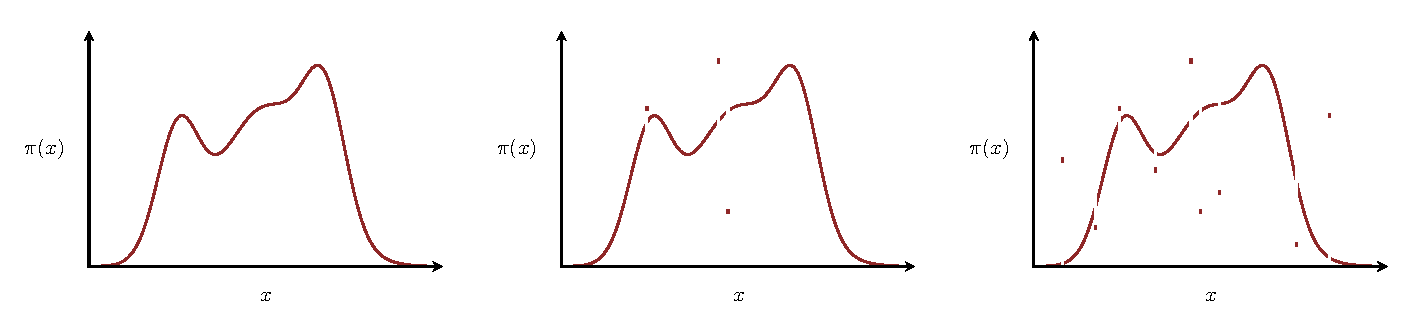
\includegraphics[width=0.95\textwidth,height=\textheight]{figures/equivalent_density_functions/equivalent_density_functions.pdf}

}

\caption{\label{fig-equivalent-density-functions}As with any density
function Lebesgue probability density functions are defined only up to
the null subsets of the reference measure; for the Lebesgue measure this
includes atomic subsets and their countable unions. All three of these
Lebesgue probability density functions are equivalent in the sense that
they define exactly the same expectation values for any expectand. One
way to break this ambiguity is to introduce an additional constraint;
for example the left probability density function is the only continuous
probability density function.}

\end{figure}

Most references take this subtlety for granted, abusing the equals sign
by writing \[
\frac{ \mathrm{d} \pi }{ \mathrm{d} \lambda}
=
\frac{ \mathrm{d} \rho }{ \mathrm{d} \lambda}
\] to mean that \[
\int_{-\infty}^{+\infty} \mathrm{d} x \,
\frac{ \mathrm{d} \pi }{ \mathrm{d} \lambda}(x)
\, f(x)
=
\int_{-\infty}^{+\infty} \mathrm{d} x \,
\frac{ \mathrm{d} \rho }{ \mathrm{d} \lambda}(x)
\, f(x)
\] for any sufficiently well-behaved expectand \(f\). Unfortunately this
sloppy notation is ubiquitous and impossible to avoid in practice.

One way to make this convention a bit more rigorous is to impose
additional constraints on the probability density functions when
possible. For example if we can can restrict consideration to
\emph{continuous} probability density functions then \[
\int_{-\infty}^{+\infty} \mathrm{d} x \,
\frac{ \mathrm{d} \pi }{ \mathrm{d} \lambda}(x)
\, f(x)
=
\int_{-\infty}^{+\infty} \mathrm{d} x \,
\frac{ \mathrm{d} \rho }{ \mathrm{d} \lambda}(x)
\, f(x)
\] usually implies point-wise equality, \[
\frac{ \mathrm{d} \pi }{ \mathrm{d} \lambda}(x)
=
\frac{ \mathrm{d} \rho }{ \mathrm{d} \lambda}(x)
\] for all \(x \in \mathbb{R}\).

Regardless we have to be careful with unstated assumptions. Directly
equating probability density functions implies either that the equality
holds only up to reference null subsets or that we're restricting
consideration to certain structured probability density functions and
not just any valid probability density functions.

The safest approach is to never forget that, unlike regular functions,
\emph{Lebesgue probability density functions do not exist on their own}.
Rather Lebesgue probability density functions \emph{always} live under
the shadow of integral signs. Anytime we see a bare probability density
function we should recognize the implied integral context.

\hypertarget{sec:visualizing}{%
\subsection{Lebesgue Probability Density Functions As
Visualizations}\label{sec:visualizing}}

Lebesgue probability density functions quantify probability
distributions by integration; for example on a real line the area under
the curve defined by a probability density function corresponds to
interval probabilities. If we train ourselves to ``integrate by eye'',
qualitatively mapping intervals to areas under a given curve, then we
can extract a wealth of information by visually examining a Lebesgue
probability density function.

For example consider two intervals \(\mathsf{I}_{1}\) and
\(\mathsf{I}_{2}\) of the same width but at different positions on a
real line. If \(\mathrm{d} \pi / \mathrm{d} \lambda (x)\) is larger for
all points in \(\mathsf{I}_{1}\) than it is for all points in
\(\mathsf{I}_{2}\) then the probability allocated to the first interval
will be larger than the probability allocated to the second interval
(Figure~\ref{fig-equal-intervals}) \[
\pi(\mathsf{I}_{1}) > \pi(\mathsf{I}_{2}).
\]

\begin{figure}

\begin{minipage}[t]{0.01\linewidth}

{\centering 

~

}

\end{minipage}%
%
\begin{minipage}[t]{0.49\linewidth}

{\centering 

\raisebox{-\height}{

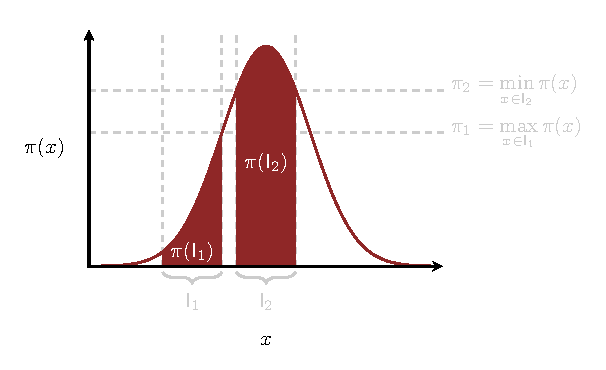
\includegraphics{figures/area_comps/equal_intervals/equal_intervals.pdf}

}

}

\subcaption{\label{fig-equal-intervals}}
\end{minipage}%
%
\begin{minipage}[t]{0.49\linewidth}

{\centering 

\raisebox{-\height}{

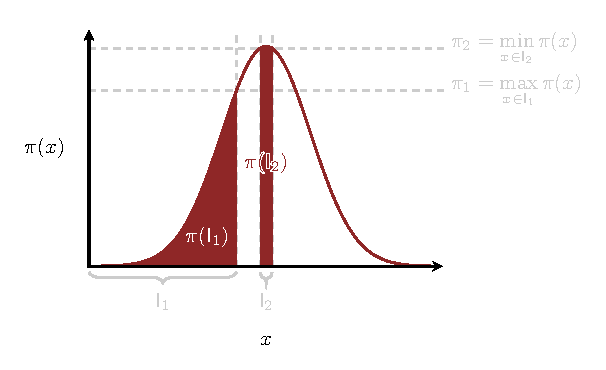
\includegraphics{figures/area_comps/unequal_intervals/unequal_intervals.pdf}

}

}

\subcaption{\label{fig-unequal-intervals}}
\end{minipage}%
%
\begin{minipage}[t]{0.01\linewidth}

{\centering 

~

}

\end{minipage}%

\caption{\label{fig-area-comps}Integrating a probability density
function by eye is not always straightforward. In particular bounds
between probability densities do not always imply bounds between
interval probabilities. (a) Here largest probability density in the
first interval, \(p_{1}\), is smaller than the smallest probability
density in the second interval, \(p_{2}\). Because the two intervals are
the same length the probability allocated to the second interval must be
larger than the probability allocated to the second interval. (b) In
this case we still have the largest probability density in the first
interval smaller than the smallest probability density in the second
interval, \(p_{1} < p_{2}\). Because the two intervals are not the same
length, however, this does not imply that
\(\pi(\mathsf{I}_{1}) < \pi(\mathsf{I}_{2})\). Indeed
\(\pi(\mathsf{I}_{1})\) is almost twice as large as
\(\pi(\mathsf{I}_{2})\)!}

\end{figure}

That said we have to take care when visually comparing intervals of
different lengths. A narrow interval can be allocated negligible
probability even if the probability density function is extremely large
everywhere within it. Similarly intervals where the probability density
function is everywhere small can still be allocated appreciable
probabilities if the interval is large enough
(Figure~\ref{fig-unequal-intervals}).

With care these visual comparisons can convey a wealth of qualitative
insights. For example if a probability density function peaks at a
single point then intervals containing the peak will tend to be
allocated larger probabilities than intervals that don't contain the
peak. In other words the probability distribution implicitly defined by
that probability density function will concentrate in the neighborhood
of that peak (Figure~\ref{fig-varying-peaks}).

\begin{figure}

\begin{minipage}[t]{0.02\linewidth}

{\centering 

~

}

\end{minipage}%
%
\begin{minipage}[t]{0.32\linewidth}

{\centering 

\raisebox{-\height}{

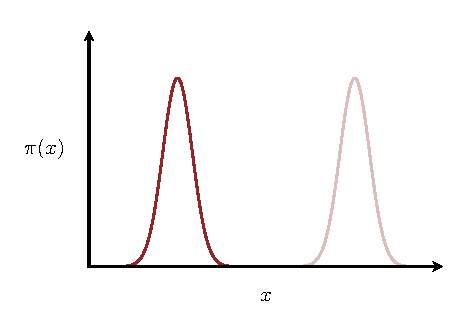
\includegraphics{figures/varying_peaks/1d/1d.pdf}

}

}

\subcaption{\label{fig-varying-peaks-1d}}
\end{minipage}%
%
\begin{minipage}[t]{0.64\linewidth}

{\centering 

\raisebox{-\height}{

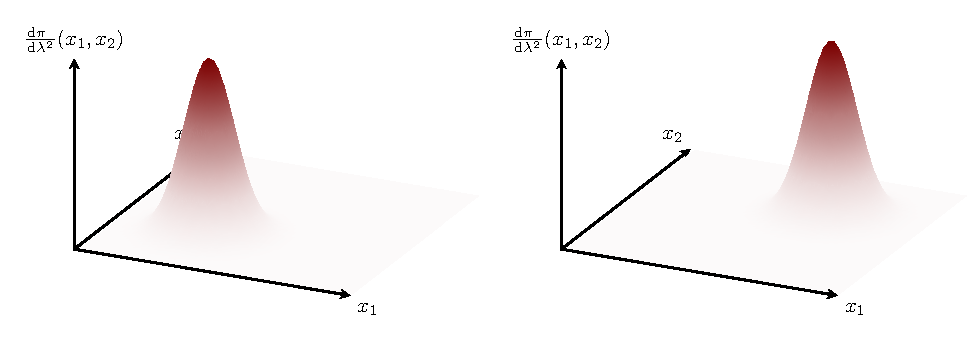
\includegraphics{figures/varying_peaks/2d/2d.pdf}

}

}

\subcaption{\label{fig-varying-peaks-2d}}
\end{minipage}%
%
\begin{minipage}[t]{0.02\linewidth}

{\centering 

~

}

\end{minipage}%

\caption{\label{fig-varying-peaks}The peaks of a Lebesgue probability
density function qualify where the corresponding probability density
function concentrates. (a) The dark red probability density function
defines a probability distribution that concentrates at smaller values
of \(x\) than the probability distribution defined by the light red
probability density function. (b) Similarly the two-dimensional
probability density function on the left defines a probability
distribution over \(\mathbb{R}^{2}\) that concentrates at values where
both \(x_{1}\) and \(x_{2}\) are small, while the one on the right
defines a probability distribution that concentrates at values where
both \(x_{1}\) and \(x_{2}\) are large.}

\end{figure}

If a probability density function exhibits multiple peaks then the
probability distribution will concentrate locally in the neighborhood of
each. Subsets falling into the gaps between these local modes will be
allocated much less probability.

The behavior of a probability density function \emph{around} a peak
qualifies how the implied probability distribution concentrates
(Figure~\ref{fig-varying-shapes}). For example if the probability
density function is wide then the concentration of probability will be
weak and if the probability density function is narrow then the
concentration will be strong. The shape of the probability density
function away from the peak qualifies the relative probability allocated
to neighborhoods around the peak compared to those away from it.
Similarly is the probability density function is asymmetric then the
concentration will be skewed.

\begin{figure}

{\centering 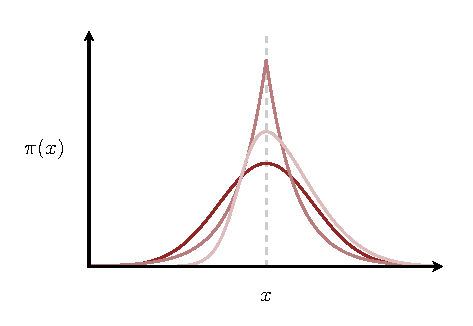
\includegraphics[width=0.6\textwidth,height=\textheight]{figures/varying_shapes/varying_shapes.pdf}

}

\caption{\label{fig-varying-shapes}The decay of a probability density
function around a peak determines how the implied probability
distribution concentrates. Here the dark red probability density
function decays symmetrically. In comparison the red probability density
function also decays symmetrically but the decay is more nuanced,
falling off quickly at first but then settling into a much slower decay
as we move away from the peak. Finally the light red probability denstiy
function decays asymmetricaly, with the implied probability distribution
allocating more probability to larger values than smaller values.}

\end{figure}

All of this said we have to be careful to not misinterpret the
point-wise behavior of a Lebesgue probability density function. For one
point-wise behavior is formally ambiguous because Radon-Nikodym
derivatives are defined only up to null subsets. More importantly
point-wise evaluations of a probability density function don't
correspond to any well-defined expectation values. Probability density
functions exist to be integrated, and visualizations of probability
density functions are useful only when they qualitatively inform how
certain integrals behave.

Finally the visualization of probability density functions is limited to
only one and two-dimensional real spaces. In higher dimensions we cannot
plot how a Lebesgue probability density function changes in every
direction at the same time.

We can plot how a probability density function varies along one and
two-dimensional cross sections of the ambient space. For example when
working on \(\mathbb{R}^{3}\) we can partically visualize a probability
density function \[
\frac{ \mathrm{d} \pi \hphantom{ {}^{3} } }{ \mathrm{d} \lambda^{3} }
(x_{1}, x_{2}, x_{3})
\] by plotting the partial evaluations \[
\frac{ \mathrm{d} \pi \hphantom{ {}^{3} } }{ \mathrm{d} \lambda^{3} }
(\tilde{x}_{1}, x_{2}, x_{3}),
\] \[
\frac{ \mathrm{d} \pi \hphantom{ {}^{3} } }{ \mathrm{d} \lambda^{3} }
(x_{1}, \tilde{x}_{2}, x_{3}),
\] and \[
\frac{ \mathrm{d} \pi \hphantom{ {}^{3} } }{ \mathrm{d} \lambda^{3} }
(x_{1}, x_{2}, \tilde{x}_{3})
\] Properly interpreting these slices, however, can be tricky. In
\textbf{Chapter Eight} we'll learn how to interpret these slices as
\emph{conditional probability density functions}.

A more effective approach in practice is to not try to visualize an
entire probability density function at once but rather investigate its
behavior when projected to lower-dimensional summaries spaces. We'll
learn how to construct these projections in the next chapter.

\hypertarget{lebesgue-probability-densities-as-limiting-interval-probabilities}{%
\subsection{Lebesgue Probability Densities As Limiting Interval
Probabilities}\label{lebesgue-probability-densities-as-limiting-interval-probabilities}}

Lebesgue probability density functions can be integrated to compute the
probability allocated to intervals. We can also use certain limiting
interval probabilities to compute Lebesgue probability densities.

To set up this latter construction let's consider a real line
\(X = \mathbb{R}\) and the interval \[
\mathsf{I} = (x_{1}, x_{1} + L ]
\] of length \(L > 0\). We can then decompose this initial interval into
\(N\) disjoint subintervals \[
\mathsf{I}_{n}
= ( x_{1} + n \, \epsilon , x_{1} + (n + 1) \, \epsilon ],
\] each of length \[
\epsilon = \frac{L}{N}.
\]

By countable additivity the probability that a probability distribution
\(\pi\) allocates to the interval \(\mathsf{I}\) is the same as the sum
of the probabilities allocated to each subinterval \(\mathsf{I}_{n}\),
\[
\pi( \, ( x_{1}, x_{1} + L ] \, )
=
\sum_{n = 0}^{N}
\pi( \, ( x_{1} + n \, \epsilon , x_{1} + (n + 1) \, \epsilon ] \, ).
\] Multiplying and dividing by the subinterval length \(\epsilon\) this
becomes \[
\pi( \, ( x_{1}, x_{1} + L ] \, )
=
\sum_{n = 0}^{N} \epsilon \cdot
\frac{
\pi( \, ( x_{1} + n \, \epsilon, x_{1} + (n + 1) \, \epsilon ] \, )
}{ \epsilon }.
\]

This, however, is exactly the setup for a Riemann integral. As the
number of subintervals increases, \(N \rightarrow \infty\), and the
length of each subinterval decreases, \(\epsilon \rightarrow 0\), the
left hand side will remain the same but the sum on the right hand side
will converge to a Riemann integral, \begin{align*}
\pi( \, ( x_{1}, x_{1} + L ] \, )
&=
\lim_{N \rightarrow \infty}
\sum_{n = 0}^{N}
\pi \left( \left( x_{1} + n \, \frac{L}{N},
                  x_{1} + (n + 1) \, \frac{L}{N} \right] \right)
\\
&=
\int_{x_{1}}^{x_{1} + L} \mathrm{d} x \, p(x),
\end{align*} with the integrand \[
p(x) = \lim_{\epsilon \rightarrow 0}
\frac{ \pi( \, ( x, x + \epsilon ] \, ) }{ \epsilon }.
\]

At the same time we can also use a probability density function between
\(\pi\) and the Lebesgue measure \(\lambda\) to compute the same
interval probability, \[
\pi( \, ( x_{1}, x_{1} + L ] \, ) =
\int_{x_{1}}^{x_{1} + L} \mathrm{d} x \,
\frac{ \mathrm{d} \pi }{ \mathrm{d} \lambda }(x).
\] Comparing these two results we can identify the Riemann integrand
with the Lebesgue probability density function, \[
\frac{ \mathrm{d} \pi }{ \mathrm{d} \lambda }(x)
\overset{\lambda}{=}
\lim_{\epsilon \rightarrow 0}
\frac{ \pi( \, ( x, x + \epsilon ] \, ) }{ \epsilon }.
\]

Note that this result relies on the choice of metric. The convergence of
a scaled interval probability to a probability density function depends
on the metric we use to define interval lengths. Different metrics will
result in different limiting values, consistent with the fact that
different metrics define different Lebesgue measures and hence different
Lebesgue probability density functions.

This result helps to explain why we have to take care with interpreting
probability densities. Lebesgue probability densities don't correspond
to interval probabilities but rather how quickly interval probabilities
change as we scan across the ambient real line; they encode
\emph{differential} information about probability allocations.
Equivalently probability density functions are endowed with units of
probability over length, not units of probability.

One practical corollary of this relationship is that we can use properly
scaled interval probabilities to \emph{approximate} probability density
functions. For small but finite \(\epsilon\) the quantity \[
\frac{ \pi( \, ( x, x + \epsilon ] \, ) }{ \epsilon }
\] approximates the Lebesgue probability density \[
\frac{ \mathrm{d} \pi }{ \mathrm{d} \lambda }(x).
\]

Consequently a histogram where the bin heights are scaled by the inverse
bin widths, \[
\frac{ \pi( \, ( x_{i}, x_{i + 1} ] \, ) }{ x_{i + 1} - x_{i} },
\] approximately visualizes a probability density function. As the bins
become narrower and narrower the scaled histogram becomes a more and
more accurate representation of the Lebesgue probability density
function (Figure~\ref{fig-histogram-approximation}).

\begin{figure}

{\centering 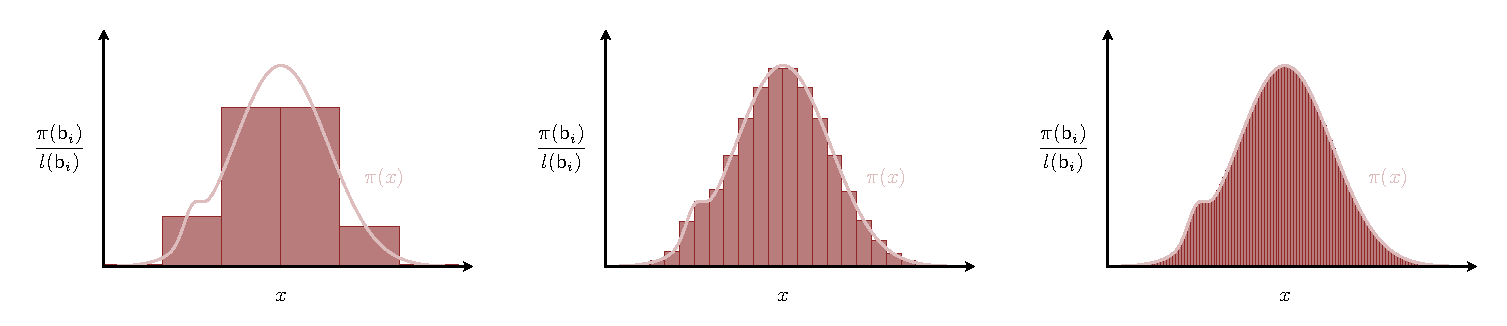
\includegraphics[width=0.96\textwidth,height=\textheight]{figures/histogram_approximation/histogram_approximation.pdf}

}

\caption{\label{fig-histogram-approximation}When we scale the bin
probabilities
\(\pi(\mathsf{b}_{i}) = \pi( \, ( x_{i}, x_{i + 1} ] \, )\) by the bin
widths \(l(\mathsf{b}_{i}) = x_{i + 1} - x_{i}\) a histogram
approximately visualizes a probability density function. As the bin
widths are decreased the approximation improves.}

\end{figure}

This approximate visualization is particularly useful when we can
compute interval probabilities but we can't evaluate the Lebesgue
probability density function. As we'll discover in the next chapter this
exact circumstance often arises when we try to project a probability
distribution from a higher-dimensional space to a lower-dimensional
space.

\hypertarget{the-normal-family-of-probability-density-functions}{%
\subsection{The Normal Family of Probability Density
Functions}\label{the-normal-family-of-probability-density-functions}}

The most convenient Lebesgue probability density functions are those
that facilitate analytic Riemann integration as much as possible. The
two-parameter \textbf{normal} family of Lebesgue probability density
functions \[
\mathrm{normal}(x; \mu, \sigma)
=
\frac{1}{\sqrt{2 \, \pi} \sigma}
\exp \left( -\frac{1}{2} \left( \frac{x - \mu}{\sigma} \right)^{2} \right),
\] where \(\mu \in \mathbb{R}\) and \(\sigma \in \mathbb{R}^{+}\), is
particularly convenient.

The two parameters \(\mu\) and \(\sigma\) directly determine the basic
shape of each normal probability density function
(Figure~\ref{fig-normal-density}). A normal probability density function
peaks at \(\mu\), which is referred to generally as a \textbf{location
parameter}. The second parameter \(\sigma\) determines how quickly the
probability density function decays as we move away from the peak; the
smaller \(\sigma\) is the narrower the density function will be. It is
known as a \textbf{scale parameter}.

\begin{figure}

{\centering 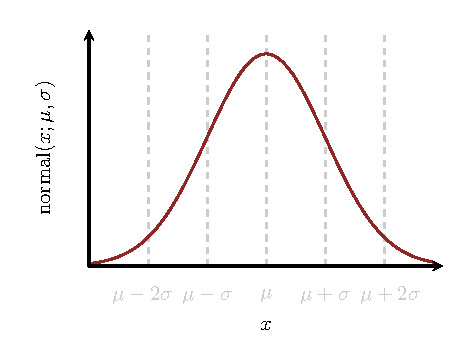
\includegraphics[width=0.6\textwidth,height=\textheight]{figures/normal/density/density.pdf}

}

\caption{\label{fig-normal-density}Every normal probability density
function peaks at the location parameter \(\mu\), with the scale
parameter \(\sigma\) controlling how quickly it decays as we move away
from the peak. The implied probability distributions allocate most of
their probability, over \(99\%\), to the interval
\((\mu - 3 \, \sigma, \mu + 3 \, \sigma)\).}

\end{figure}

Each \(\mathrm{normal}(x; \mu, \sigma)\) is referred to as a
\textbf{normal probability density function}, or just \textbf{normal
density function} for short. We might be tempted to refer to the
probability distribution defined by a normal density function as a
\textbf{normal distribution}, but this association is well-defined only
once we fix a real line and hence a particular Lebesgue measure. Because
the same normal density function will define different probability
distributions on different real lines I try to avoid terms like ``normal
distribution''.

The conventions I've used here are common, but no means standard. For
example in some fields this family is described as ``Gaussian'' in honor
of Carl Friedrich Gauss who first introduced it. Moreover there are
multiple, equivalent ways to parameterize the family including
\begin{align*}
\mathrm{normal}(x; \mu, v)
&=
\frac{1}{\sqrt{2 \, \pi \, v}}
\exp \left( -\frac{1}{2 \, v} \left( x - \mu \right)^{2} \right),
\\
\mathrm{normal}(x; \mu, \tau)
&=
\sqrt{ \frac{\tau}{2 \, \pi} }
\exp \left( -\frac{\tau}{2} \left( x - \mu \right)^{2} \right),
\end{align*} and even \[
\mathrm{normal}(x; \eta_{1}, \eta_{2})
=
\sqrt{ \frac{-\eta_{2}}{\pi} }
\exp \left(  \eta_{1} \, x + \eta_{2} \, x^{2}
           + \frac{\eta_{1}^{2}}{4 \, \eta_{2}^{2}} \right).
\] Each of these parameterizations can be convenient in certain
circumstances, but the initial parameterization defined above tends to
the most useful for practical applications

The integrals \[
\int_{-\infty}^{+\infty} \mathrm{d} x \,
\mathrm{normal}(x; \mu, \sigma) \, f(x)
\] that define expectation values are particularly nice, at least as far
as integrals go. That isn't to say that the integrals are easy to
evaluate but rather that they many of them actually admit closed-form
solutions, which is pretty miraculous when it comes to integrals. For
those twisted individuals who fancy a good integral calculation, myself
included, I've included those calculations in the
\href{@sec:appendix}{Appendix}. Everyone else can take these results at
face value.

For example we can verify that each probability density function in the
normal family is properly normalized with the integral \begin{align*}
\mathrm{normal}(\mathbb{R}; \mu, \sigma)
&=
\int_{-\infty}^{+\infty} \mathrm{d} x \,
\mathrm{normal}(x; \mu, \sigma)
\\
&=
\int_{-\infty}^{+\infty} \mathrm{d} x \,
\frac{1}{\sqrt{2 \, \pi} \sigma}
\exp \left( -\frac{1}{2} \left( \frac{x - \mu}{\sigma} \right)^{2} \right)
\\
&=
1.
\end{align*}

Similarly we can compute the mean of the probability distribution
implied by each normal density function, \begin{align*}
\mathbb{M}(\mu, \sigma)
&=
\mathbb{E}_{\mathrm{normal}}[ \iota; \mu, \sigma ]
\\
&=
\int_{-\infty}^{+\infty} \mathrm{d} x \,
\mathrm{normal}(x; \mu, \sigma) \, x
\\
&=
\int_{-\infty}^{+\infty} \mathrm{d} x \,
\frac{1}{\sqrt{2 \, \pi} \sigma}
\exp \left( -\frac{1}{2} \left( \frac{x - \mu}{\sigma} \right)^{2} \right)
\, x
\\
&=
\mu.
\end{align*} The parameter \(\mu\) determines not just the peak of each
normal probability density function but also the mean of each
corresponding probability distribution. Because of this \(\mu\) is
sometimes referred to as a \textbf{mean parameter}.

With even more mathematical elbow grease we can show that the variance
is given by \begin{align*}
\mathbb{V}(\mu, \sigma)
&=
\mathbb{E}_{\mathrm{normal}}[ (\iota - \mathbb{M}(\mu, \sigma))^{2}; \mu, \sigma ]
\\
&=
\mathbb{E}_{\mathrm{normal}}[ (\iota - \mu)^{2}; \mu, \sigma ]
\\
&=
\int_{-\infty}^{+\infty} \mathrm{d} x \,
\mathrm{normal}(x; \mu, \sigma) \, (x - \mu)^{2}
\\
&=
\int_{-\infty}^{+\infty} \mathrm{d} x \,
\frac{1}{\sqrt{2 \, \pi} \sigma}
\exp \left( -\frac{1}{2} \left( \frac{x - \mu}{\sigma} \right)^{2} \right)
\, (x - \mu)^{2}
\\
&=
\sigma^{2}.
\end{align*} As we increase \(\sigma\) the normal probability density
functions widen and the variance of the implied probability
distributions increases.

Normal probability density functions can also be used to evaluate the
cumulative distribution function corresponding to the implicitly-defined
probability distributions, \begin{align*}
\Pi_{\text{normal}}(x; \mu, \sigma)
&=
\text{normal}( \, (-\infty, x]; \mu, \sigma \, )
\\
&=
\mathbb{E}_{\mathrm{normal}}[ I_{(-\infty, x]}; \mu, \sigma ]
\\
&=
\int_{-\infty}^{+\infty} \mathrm{d} x' \,
\mathrm{normal}(x'; \mu, \sigma) \, I_{(-\infty, x]}(x')
\\
&=
\int_{-\infty}^{x} \mathrm{d} x' \,
\mathrm{normal}(x'; \mu, \sigma)
\\
&=
\frac{1}{2}
+
\frac{1}{2} \,
\mathrm{erf} \left( \frac{x - \mu}{\sqrt{2} \, \sigma} \right),
\end{align*} where \[
\mathrm{erf} (x)
\frac{2}{\sqrt{\pi}}
\int_{0}^{ x } \mathrm{d} t \, \exp \left( -t^{2} \right)
\] is known as the \textbf{error function}.

Conveniently the error function, if not the normal cumulative
distribution functions themselves, are available in most programming
languages. This allows us directly compute interval probabilities by
subtracting cumulative probabilities
(Figure~\ref{fig-normal-interval-prob}), \[
\text{normal}( \, (x_{1}, x_{2} ] \, ; \mu, \sigma )
=
\frac{1}{2} \, \left(
  \mathrm{erf} \left( \frac{x_{2} - \mu}{\sqrt{2} \, \sigma} \right)
- \mathrm{erf} \left( \frac{x_{1} - \mu}{\sqrt{2} \, \sigma} \right)
\right).
\]

\begin{figure}

{\centering 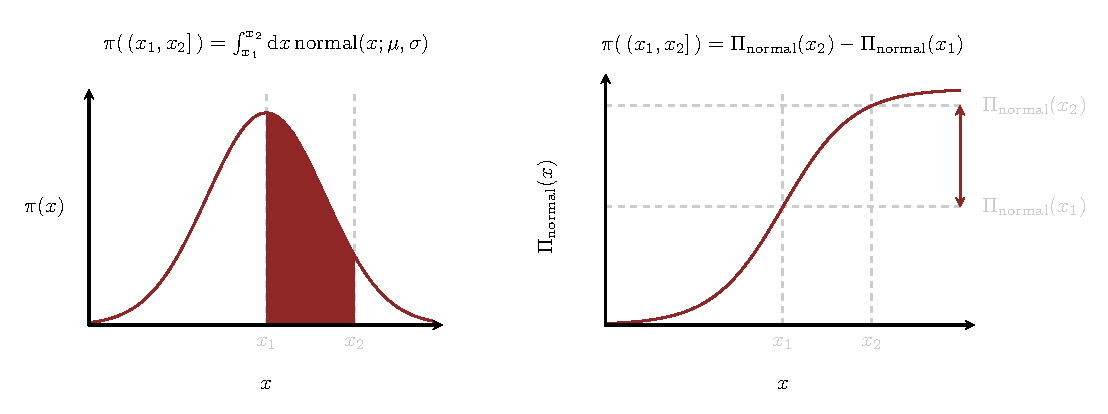
\includegraphics[width=0.9\textwidth,height=\textheight]{figures/normal/interval_prob/interval_prob.pdf}

}

\caption{\label{fig-normal-interval-prob}The normal cumulative
distribution functions \(\Pi_{\text{normal}}(x; \mu, \sigma)\) provide
another way to compute interval probabilities. In addition to
integrating under the curve defined by a normal probability density
function we can also subtract the cumulative probabilities at the
interval boundaries.}

\end{figure}

\hypertarget{other-useful-probability-density-functions}{%
\section{Other Useful Probability Density
Functions}\label{other-useful-probability-density-functions}}

Most of applications of probability theory that we will tackle in this
book will use probability distributions that are absolutely continuous
with respect to a counting measure or a Lebesgue measure and implemented
with appropriate probability density functions. There are a few
exceptions, however, that we will occasionally need to accommodate.

\hypertarget{singular-probability-density-functions}{%
\subsection{Singular Probability Density
Functions}\label{singular-probability-density-functions}}

On any measurable space where the atomic subsets are measurable we can
always define a \emph{singular} probability distribution \(\delta_{x'}\)
that concentrates all probability on a single point \(x' \in X\), \[
\delta_{x}(\mathsf{x}) =
\left\{
\begin{array}{rr}
1, & x' \in \mathsf{x} \\
0, & x' \notin \mathsf{x}
\end{array}
\right. .
\] More generally because only a single point contributes we can define
expectation values by the point-wise evaluation of the expectand, \[
\mathbb{E}_{\delta_{x}} [f] = f(x').
\] These probability distributions are known as \textbf{Dirac
distributions}.

Because \(\delta_{x'}(\{ x' \}) = 1\) the atomic subset \(\{ x' \}\) is
\emph{not} a null subset with respect to \(\delta_{x'}\). Consequently
Dirac distributions are not absolutely continuous with respect to any
reference measure that allocates vanishing probability to the atomic
subsets. In particular singular probability distributions on real lines
are not absolutely continuous with respect to the Lebesgue measure, and
we \emph{cannot represent them with ordinary functions}!

For example if a probability density function existed then we should be
able to engineer a function \(\delta(x - x')\) such that \[
f(x')
= \mathbb{E}_{\delta_{x'}} [f]
= \mathbb{I}_{\lambda} [ \delta(\cdot - x') \cdot f]
= \int_{-\infty}^{\infty} \mathrm{d} x \, \delta(x - x') \, f(x)
\] for any expectand \(f: \mathbb{R} \rightarrow \mathbb{R}\). How could
we achieve this behavior?

Well if the hypothetical density function \(\delta(x - x')\)
concentrated around \(x'\) then the integrals would also concentrate
around \(f(x')\). For example integrals of normal probability density
functions centered at \(x'\) approximate the desired behavior better and
better as the scale becomes smaller and smaller
(Figure~\ref{fig-singular-density}).

\begin{figure}

\begin{minipage}[t]{0.05\linewidth}

{\centering 

~

}

\end{minipage}%
%
\begin{minipage}[t]{0.45\linewidth}

{\centering 

\raisebox{-\height}{

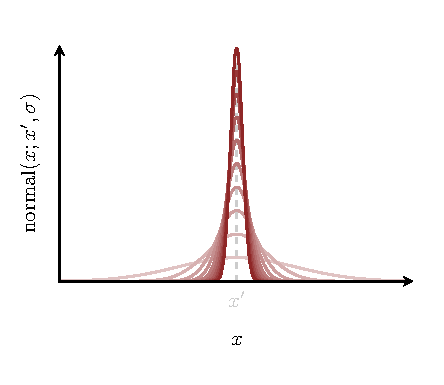
\includegraphics{figures/singular_density/narrowing_normals/narrowing_normals.pdf}

}

}

\subcaption{\label{fig-narrowing-normals}}
\end{minipage}%
%
\begin{minipage}[t]{0.45\linewidth}

{\centering 

\raisebox{-\height}{

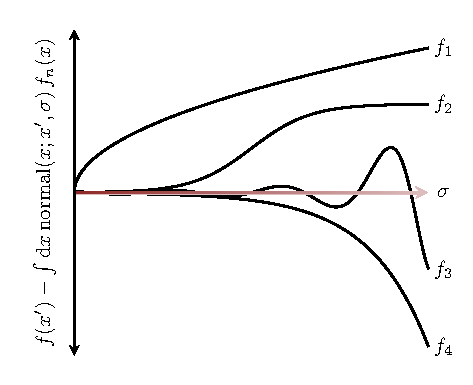
\includegraphics{figures/singular_density/converging_expectations/converging_expectations.pdf}

}

}

\subcaption{\label{fig-converging-expectations}}
\end{minipage}%
%
\begin{minipage}[t]{0.05\linewidth}

{\centering 

~

}

\end{minipage}%

\caption{\label{fig-singular-density}As they become narrower and
narrower normal probability density functions start to behave like a
hypothetical singular density function. (a) In the limit
\(\sigma \rightarrow 0\) the normal probability density functions
centered at \(\mu = x'\) converge to an infinitely narrow spike at
\(x'\). (b) At the same the expectation values of all expectands \(f\)
coverge to the point evaluations \(f(x')\).}

\end{figure}

In the limit \(\sigma \rightarrow 0\) the normal probability density
functions reduce to an infinitely high spike at the mean, \[
\lim_{\sigma \rightarrow 0}
\frac{1}{\sqrt{2 \, \pi} \sigma}
\exp \left( -\frac{1}{2} \left( \frac{x' - x}{\sigma} \right)^{2} \right)
=
\left\{
\begin{array}{rr}
\infty, & x' = x \\
0, & x' \ne x
\end{array}
\right. .
\] Perhaps we can we define \(\delta(x - x')\) by this spike?

Unfortunately this intuition doesn't quite work out. Remember that
probability density functions can be modified at a null subset of input
points without affecting their integrals. Because \(\{ x' \}\) is a
Lebesgue null subset this implies that our infinite spike should be
equivalent to a function \(z\) that returns zero for \emph{all} inputs,
\[
\mathbb{I}_{\lambda} [ \delta(\cdot - x') \cdot f]
=
\mathbb{I}_{\lambda} [ z \cdot f]
=
\mathbb{I}_{\lambda} [ z ].
\] Unfortunately this results in an ill-defined integral, \[
\mathbb{I}_{\lambda} [ z ]
= \int_{-\infty}^{+\infty} \mathrm{d} x \, 0
= 0 \cdot \infty.
\] that contradicts the desired behavior \[
\mathbb{I}_{\lambda} [ \delta(\cdot - x') \cdot f] = f(x').
\] \emph{We cannot define a function that can scale a Lebesgue measure
into a singular Dirac distribution}. Of course this is what the failure
of absolutely continuity was trying to tell us in the first place!

Because the expectation values are trivial to compute, working with a
singular probability distribution directly is straightforward. The lack
of a well-defined singular density function, however, can be awkward
when we're exclusively using probability density functions to specify
every other probability distribution of interest.

One way to get around this issue is to just \emph{define} an object
\(\delta\) called the \textbf{Dirac delta function} that satisfies \[
f(0)
= \int_{-\infty}^{\infty} \mathrm{d} x \, \delta(x) \, f(x)
\] for all functions \(f : \mathbb{R} \rightarrow \mathbb{R}\).
Frustratingly contrary to the name, \(\delta\) \emph{is not a function}
but rather what mathematicians call a \textbf{generalized function}.
Fortunately these technicalities don't matter so long as we only ever
use the formal integral definition in calculations.

For example consider an application where we want to \emph{inflate} the
probability allocated to the atomic subset \(\{ x' \}\) from \(0\) to
\(0 < \gamma \le 1\), breaking absolute continuity with respect to the
Lebesgue measure in the process. We can achieve this with a
\textbf{mixture probability distribution} that combines a Dirac
distribution \(\delta_{x'}\) with the initial probability distribution
\(\pi\) that is absolutely continuous with respect to the Lebesgue
measure, \[
\rho = \gamma \, \delta_{x'} + (1 - \gamma) \, \pi.
\] This mixture distribution defines the subset allocations
\begin{align*}
\rho(\mathsf{x})
&=
  \gamma \, \delta_{x'}(\mathsf{x})
+ (1 - \gamma) \, \pi(\mathsf{x})
\\
&=
\left\{
\begin{array}{rr}
\gamma + (1 - \gamma) \, \pi(\mathsf{x}), & x' \in \mathsf{x} \\
(1 - \gamma) \, \pi(\mathsf{x}), & x' \notin \mathsf{x}
\end{array}
\right.
\end{align*} and the expectation values \begin{align*}
\mathbb{E}_{\rho}[f]
&=
  \gamma \, \mathbb{E}_{\delta_{x'}}[f]
+ (1 - \gamma) \, \mathbb{E}_{\pi}[f]
\\
&=
\gamma \, f(x') + (1 - \gamma) \, \mathbb{E}_{\pi}[f].
\end{align*}

Using the Dirac delta function we can \emph{heuristicaly} represent this
mixture distribution as \[
\frac{\mathrm{d} \rho}{\mathrm{d} \lambda}(x)
=   \gamma \, \delta(x - x')
  + (1 - \gamma) \, \frac{\mathrm{d} \pi}{\mathrm{d} \lambda}(x)
\] where all expectation values are calculated as \begin{align*}
\mathbb{E}_{\rho}[f]
&=
\int_{-\infty}^{\infty} \mathrm{d} x \,
\frac{\mathrm{d} \rho}{\mathrm{d} \lambda}(x) \, f(x)
\\
&=
\int_{-\infty}^{\infty} \mathrm{d} x \,
\left( \gamma \, \delta(x - x') +
       (1 - \gamma) \, \frac{\mathrm{d} \pi}{\mathrm{d} \lambda}(x)(x)
\right) \, f(x)
\\
&=
\gamma \, \int_{-\infty}^{\infty} \mathrm{d} x \, \delta(x - x') \, f(x)
+ (1 - \gamma) \,
\int_{-\infty}^{\infty} \mathrm{d} x \,
\frac{\mathrm{d} \pi}{\mathrm{d} \lambda}(x) \, f(x)
\\
&=
\gamma \, f(x')
+ (1 - \gamma) \,
\int_{-\infty}^{\infty} \mathrm{d} x \,
\frac{\mathrm{d} \pi}{\mathrm{d} \lambda}(x) \, f(x)
\\
&=
\gamma \, f(x') + (1 - \gamma) \, \mathbb{E}_{\pi}[f].
\end{align*}

If we restrict consideration to continuous probability density functions
then we can visualize this mixture density function
\(\mathrm{d} \rho / \mathrm{d} \lambda\) as a continuous base density
function \(\mathrm{d} \pi / \mathrm{d} \lambda\) with a single
discontinuity at \(x'\) (Figure~\ref{fig-inflation}). Without this
restriction, however, visualizations like this are ambiguous because
\(\mathrm{d} \pi / \mathrm{d} \lambda\) is defined only up to subsets of
null Lebsegue measure.

\begin{figure}

{\centering 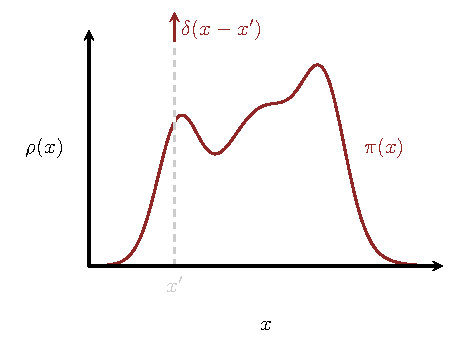
\includegraphics[width=0.6\textwidth,height=\textheight]{figures/singular_density/inflation/inflation.pdf}

}

\caption{\label{fig-inflation}One way to visually represent the mixture
of a base probability distribution with a singular probability
distribution is to inflate the base probability density function with an
infinite spike. This visualization is well-defined, however, only if we
assume a continuous probability density function for the base
probability distribution.}

\end{figure}

Because of all of this delicate mathematical baggage the Dirac delta
``function'' requires care when using in practice. That said the
compact, dare I say elegant, probability density function descriptions
it enables is often worth the added subtlety.

\hypertarget{geometric-probability-density-functions}{%
\subsection{Geometric Probability Density
Functions}\label{geometric-probability-density-functions}}

Real spaces adequately model many phenomena that arise in practical
applications, but by no means all of them. In some cases we will need to
consider continuous spaces that look like a real spaces \emph{locally}
but exhibit different shapes \emph{globally} (Figure~\ref{fig-circle}).
These include for example spheres, torii, and even more foreign spaces.
Mathematically these spaces, along with real spaces, are collectively
known as \textbf{manifolds}.

\begin{figure}

\begin{minipage}[t]{0.20\linewidth}

{\centering 

~

}

\end{minipage}%
%
\begin{minipage}[t]{0.60\linewidth}

{\centering 

\raisebox{-\height}{

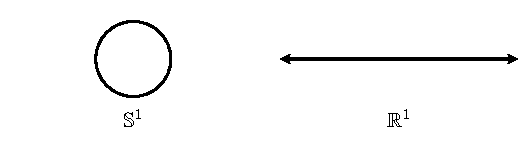
\includegraphics{figures/circle_vs_line/far/far.pdf}

}

}

\subcaption{\label{fig-circle-far}}
\end{minipage}%
%
\begin{minipage}[t]{0.20\linewidth}

{\centering 

~

}

\end{minipage}%
\newline
\begin{minipage}[t]{0.20\linewidth}

{\centering 

~

}

\end{minipage}%
%
\begin{minipage}[t]{0.60\linewidth}

{\centering 

\raisebox{-\height}{

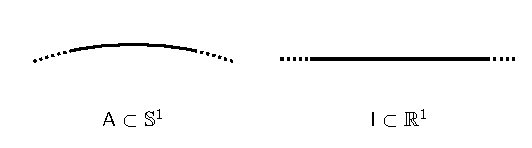
\includegraphics{figures/circle_vs_line/close/close.pdf}

}

}

\subcaption{\label{fig-circle-close}}
\end{minipage}%
%
\begin{minipage}[t]{0.20\linewidth}

{\centering 

~

}

\end{minipage}%

\caption{\label{fig-circle}A circle \(\mathbb{S}^{1}\) is an example of
a manifold. (a) Globally the space defined by a circle is distinct from
the space defined by a real line. (b) If we zoom in, however, the local
behavior of the circle is equivalent to the local behavior of a real
line.}

\end{figure}

One nice feature of manifolds is that we can always equip them with
consistent metric structures. A chosen metric then allows us to define a
compatible uniform measure that emulates many of the features of the
Lebesgue measure on real spaces. In particular these uniform measures
serve as natural reference measures on which we can build many useful
probability distributions.

For example we can equip a circle \(S^{1}\) with a metric that endows
angular intervals with a notion of length
(Figure~\ref{fig-circle-metric}). We can then define a uniform measure
that allocates the same measure to every angular interval of the same
length (Figure~\ref{fig-circle-measure}).

\begin{figure}

\begin{minipage}[t]{0.15\linewidth}

{\centering 

~

}

\end{minipage}%
%
\begin{minipage}[t]{0.35\linewidth}

{\centering 

\raisebox{-\height}{

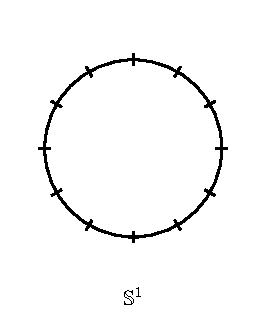
\includegraphics{figures/uniform_circle/metric/metric.pdf}

}

}

\subcaption{\label{fig-circle-metric}}
\end{minipage}%
%
\begin{minipage}[t]{0.35\linewidth}

{\centering 

\raisebox{-\height}{

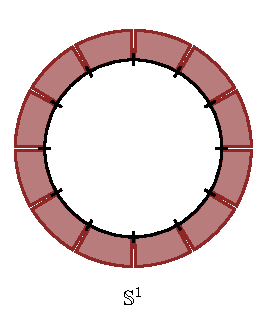
\includegraphics{figures/uniform_circle/measure/measure.pdf}

}

}

\subcaption{\label{fig-circle-measure}}
\end{minipage}%
%
\begin{minipage}[t]{0.15\linewidth}

{\centering 

~

}

\end{minipage}%

\caption{\label{fig-circle}Manifolds like the circle can be equipped
with metrics, and uniform measures compatible with that metric
structure. (a) A metric endows each angular interval with a length. (b)
We can then define a uniform measure that allocates to each angular
interval a measure equal to its length.}

\end{figure}

Another important consequence of this construction is that, similar to
the Lebesgue measure, these uniform measures allocate zero measure to
every atomic subset. Consequently any probability distribution over
\(S^{1}\) that also allocates vanishing probability to the atomic
subsets will be absolutely continuous to these uniform measures. This
allows us to define \textbf{circular probability density functions} \[
p : \mathbb{S}^{1} \rightarrow \mathbb{R}^{+}
\] to represent each of these absolutely continuous probability
distributions (Figure~\ref{fig-circular-density-functions}).

\begin{figure}

{\centering 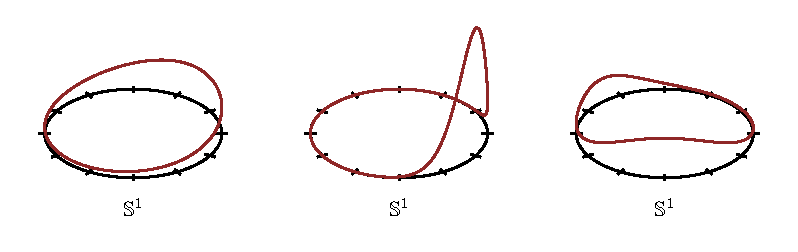
\includegraphics[width=0.9\textwidth,height=\textheight]{figures/circular_density_functions/circular_density_functions.pdf}

}

\caption{\label{fig-circular-density-functions}Sufficiently nice
probability distributions on a circle \(\mathbb{S}^{1}\) can be
represented by circular probability density functions
\(p : \mathbb{S}^{1} \rightarrow \mathbb{R}^{+}\). Similar to Lebesgue
probability density functions these circular probability density
functions visualize a host of qualitative behaviors, such as where and
how the implied probability distributions concentrate.}

\end{figure}

We have to take care, however, not to confuse these circular probability
density functions with Lebesgue probability density functions. In
particular expectation values \[
\mathbb{E}_{\pi}[f] = \mathbb{I}_{\nu}[p \cdot f]
\] are not implemented with classic Riemann integration but rather a
more general \textbf{manifold integration} that is not implemented in
the same way.

That said sometimes there are work arounds. For example removing a point
\(x' \in \mathbb{S}^{1}\) from the circle defines a new space
\(\mathbb{S}^{1} \setminus x'\). Circular probability distributions,
circular probability density functions, and circular expectands
\(f : \mathbb{S} \rightarrow \mathbb{R}\) on the circle all define
corresponding objects on this excised space. Once we've removed the
point we can then unroll and stretch out \(\mathbb{S}^{1} \setminus x'\)
into a real line \(\mathbb{R}\), taking all of the probabilistic objects
along with us (Figure~\ref{fig-cutting-circles}).

In general expectation values on the initial circular probability space
will be different from the expectation values on the excised probability
space. If \(\{ x' \}\) is a null subset, however, then they will be the
same, \[
\mathbb{E}_{\pi}[f]
= \mathbb{I}_{\nu}[p \cdot f]
= \mathbb{I}_{\nu'}[p' \cdot f']
= \mathbb{I}_{\nu''}[p'' \cdot f''],
\] where no ticks denotes objects on \(\mathbb{S}^{1}\), one tick
denotes objects on \(\mathbb{S}^{1} \setminus \mathbb{R}\), and two
ticks denotes objects on \(\mathbb{R}\).

To summarize, by removing a point from the circle we can implement
circular expectation values with classic Riemann integrals. Not every
cut point, however, will be as convenient as others. Cutting the circle
away from where the initial probability density function concentrates
results in a well-behaved, unimodal Lebesgue probability density
function (Figure~\ref{fig-cutting-circles-good}). On the other hand
cutting near the centrality of the probability density function results
in a Lebesgue probability density function with two peaks at relatively
extreme values, which can easily frustrate integral calculations
(Figure~\ref{fig-cutting-circles-bad}).

\begin{figure}

\begin{minipage}[t]{0.05\linewidth}

{\centering 

~

}

\end{minipage}%
%
\begin{minipage}[t]{0.45\linewidth}

{\centering 

\raisebox{-\height}{

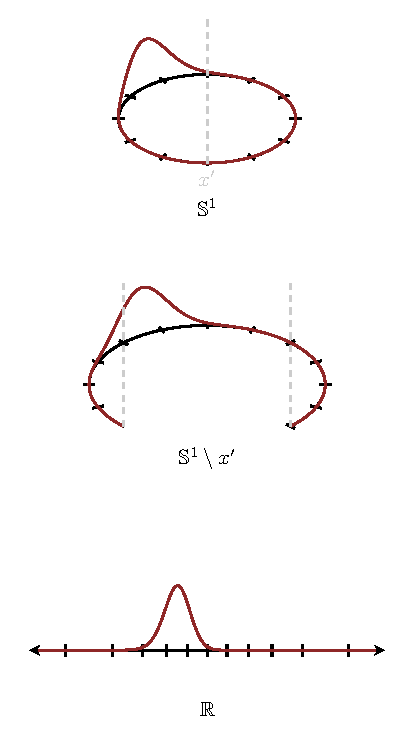
\includegraphics{figures/cutting_circles/good/good.pdf}

}

}

\subcaption{\label{fig-cutting-circles-good}}
\end{minipage}%
%
\begin{minipage}[t]{0.45\linewidth}

{\centering 

\raisebox{-\height}{

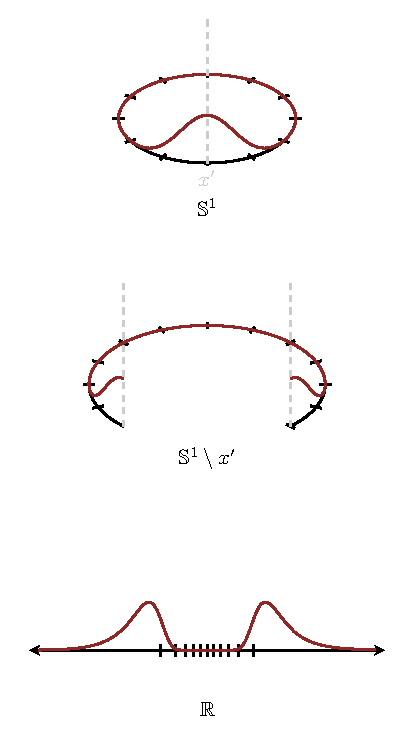
\includegraphics{figures/cutting_circles/bad/bad.pdf}

}

}

\subcaption{\label{fig-cutting-circles-bad}}
\end{minipage}%
%
\begin{minipage}[t]{0.05\linewidth}

{\centering 

~

}

\end{minipage}%

\caption{\label{fig-cutting-circles}Probabilistic computations on a
circle can be transformed into integrals on a real line with a little
bit of surgery. Removing a point \(x'\) from a circle \(\mathbb{S}^{1}\)
gives the space \(\mathbb{S}^{1} \setminus x'\) which can be unrolled
and stretched out into a real line \(\mathbb{R}\). Because its removes
only a null subset this surgery doesn't affect integrals, allowing us to
compute circular expectation values with Riemann integrals on
\(\mathbb{R}\). Which point we remove, however, can have a strong
influence no how difficult those Riemann integrals are. (a) Cutting the
circle at a point around which little probability is allocated results
in a well-behaved Lebesgue probability density function that facilitates
integration. (b) On the other hand cutting at a point around which a
substantial amount of probability is allocated results in a more
pathological Lebesgue probability density function that frustrates
integration.}

\end{figure}

If we don't know where the initial circular probability density function
concentrates then we won't know where to make a good cut, and we can end
up with a difficult Lebesgue probability density function that doesn't
actually get us any closer to a completed calculation. The subtle
relationship between circular probability density functions, let alone
other, more complicated manifold probability density functions, and
Lebesgue probability density functions is dark and full of terrors. To
avoid computational problems, or worse corrupting the target expectation
values, we need to be very careful when working on these more
sophisticated spaces.

\hypertarget{conclusion}{%
\section{Conclusion}\label{conclusion}}

Because they provide a straightforward way to implement probability
distributions in practice, probability density functions are absolutely
critical in transitioning probability theory from abstract mathematics
to a viable tool for applied practice. That said because they define
probability distributions only in the context of integrals informed by a
given reference measure they are not without their subtleties. When we
ignore this context we become prone to incorrect interpretations and
implementations which then results in inconsistent applications of the
underlying probability theory.

\hypertarget{acknowledgements}{%
\section*{Acknowledgements}\label{acknowledgements}}
\addcontentsline{toc}{section}{Acknowledgements}

A very special thanks to everyone supporting me on Patreon: Adam
Fleischhacker, Adriano Yoshino, Alan Chang, Alessandro Varacca,
Alexander Noll, Alexander Petrov, Alexander Rosteck, Anders Valind,
Andrea Serafino, Andrew Mascioli, Andrew Rouillard, Andrew Vigotsky,
Angie\_Hyunji Moon, Ara Winter, Austin Rochford, Austin Rochford,
Avraham Adler, Ben Matthews, Ben Swallow, Benjamin Glemain, Benoit
Essiambre, Bradley Kolb, Brandon Liu, Brendan Galdo, Brynjolfur Gauti
Jónsson, Cameron Smith, Canaan Breiss, Cat Shark, Charles Naylor, Chase
Dwelle, Chris, Chris Jones, Christopher Mehrvarzi, Colin Carroll, Colin
McAuliffe, Damien Mannion, Damon Bayer, dan mackinlay, Dan Muck, Dan W
Joyce, Dan Waxman, Dan Weitzenfeld, Daniel Edward Marthaler, Darshan
Pandit, Darthmaluus , David Burdelski, David Galley, David Wurtz, Denis
Vlašiček, Doug Rivers, Dr.~Jobo, Dr.~Omri Har Shemesh, Dylan Maher, Ed
Cashin, Edgar Merkle, Eric LaMotte, Erik Banek, Ero Carrera, Eugene
O'Friel, Felipe González, Fergus Chadwick, Finn Lindgren, Florian
Wellmann, Francesco Corona, Geoff Rollins, Greg Sutcliffe, Guido Biele,
Hamed Bastan-Hagh, Haonan Zhu, Hector Munoz, Henri Wallen, hs, Hugo
Botha, Håkan Johansson, Ian Costley, Ian Koller, idontgetoutmuch,
Ignacio Vera, Ilaria Prosdocimi, Isaac Vock, J, J Michael Burgess, Jair
Andrade, James C, James Hodgson, James Wade, Janek Berger, Jason Martin,
Jason Pekos, Jason Wong, Jeff Burnett, Jeff Dotson, Jeff Helzner,
Jeffrey Erlich, Jesse Wolfhagen, Jessica Graves, Joe Wagner, John
Flournoy, Jonathan H. Morgan, Jonathon Vallejo, Joran Jongerling, Josh
Weinstock, Joshua Duncan, Joshua Griffith, JU, Justin Bois, Karim
Naguib, Karim Osman, Kejia Shi, Kristian Gårdhus Wichmann, Kádár András,
Lars Barquist, lizzie , LOU ODETTE, Luís F, Marcel Lüthi, Marek
Kwiatkowski, Mark Donoghoe, Markus P., Martin Modrák, Matt Moores, Matt
Rosinski, Matthew, Matthew Kay, Matthieu LEROY, Mattia Arsendi, Maurits
van der Meer, Michael Colaresi, Michael DeWitt, Michael Dillon, Michael
Lerner, Mick Cooney, Márton Vaitkus, N Sanders, Nathaniel Burbank, Nic
Fishman, Nicholas Clark, Nicholas Cowie, Nick S, Nicolas Frisby, Octavio
Medina, Oliver Crook, Olivier Ma, Patrick Kelley, Patrick Boehnke, Pau
Pereira Batlle, Peter Smits, Pieter van den Berg , ptr, Putra Manggala,
Ramiro Barrantes Reynolds, Ravin Kumar, Raúl Peralta Lozada, Riccardo
Fusaroli, Richard Nerland, Robert Frost, Robert Goldman, Robert kohn,
Robin Taylor, Ross McCullough, Ryan Grossman, Rémi , S Hong, Scott
Block, Sean Pinkney, Sean Wilson, Sergiy Protsiv, Seth Axen, shira,
Simon Duane, Simon Lilburn, sssz, Stan\_user, Stefan, Stephanie
Fitzgerald, Stephen Lienhard, Steve Bertolani, Stew Watts, Stone Chen,
Susan Holmes, Svilup, Sören Berg, Tao Ye, Tate Tunstall, Tatsuo Okubo,
Teresa Ortiz, Thomas Lees, Thomas Vladeck, Tiago Cabaço, Tim Radtke,
Tobychev , Tom McEwen, Tony Wuersch, Utku Turk, Virginia Fisher, Vitaly
Druker, Vladimir Markov, Wil Yegelwel, Will Farr, Will Tudor-Evans,
woejozney, yolhaj , Zach A, Zad Rafi, and Zhengchen Cai.

\hypertarget{sec:appendix}{%
\section*{Appendix: Sums and Integrals}\label{sec:appendix}}
\addcontentsline{toc}{section}{Appendix: Sums and Integrals}

Probability density functions allow us to compute expectation values
using explicit mathematical operations, in particular summation when
working with a counting reference measure and Riemann integration when
working with a Lebesgue reference measure. Just because these operations
are explicit, however, doesn't mean that they're straightforward.

Deriving analytic results for even the most convenient summations and
integrals can require a substantial amount of experience with
mathematical techniques, and in many cases tricks that seem to come out
of nowhere. For those who are curious about these techniques this
appendix gathers full calculations for the Poisson and normal results
that we used in this chapter.

Note that these calculations will absolutely not be necessary for
keeping up with future chapters. Indeed in most applications we will
take advantage of other computational tools that don't require these
kinds of onerous calculations at all.

\hypertarget{poisson-summations}{%
\subsection{Poisson Summations}\label{poisson-summations}}

Let's warm up with some summations.

The normalization of each Poisson probability mass function is given by
\begin{align*}
\mathrm{Poisson}(X; \lambda)
&= \mathbb{E}_{\mathrm{Poisson}}[ I_{X}; \lambda ]
\\
&= \mathbb{I}_{\chi}[ \mathrm{Poisson}( ; \lambda) \cdot I_{X} ]
\\
&= \sum_{n = 0}^{\infty} \mathrm{Poisson}(n; \lambda) \cdot 1
\\
&= \sum_{n = 0}^{\infty} \frac{ \lambda^{n} e^{-\lambda} }{ n! }
\\
&= e^{-\lambda} \sum_{n = 0}^{\infty} \frac{ \lambda^{n} }{ n! }.
\end{align*} This summation, however, is just the power series
definition for the exponential function, \[
e^{x} = \sum_{n = 0}^{\infty} \frac{ x^{n} }{ n! }.
\] Consequently \begin{align*}
\mathrm{Poisson}(X; \lambda)
&= e^{-\lambda} \sum_{n = 0}^{\infty} \frac{ \lambda^{n} }{ n! }
\\
&= e^{-\lambda} e^{\lambda}
\\
&= 1,
\end{align*} as required.

Similarly the mean for each Poisson probability distribution is given by
\begin{align*}
\mathbb{M}(\lambda)
&= \mathbb{E}_{\mathrm{Poisson}} [ \iota ; \lambda ]
\\
&= \mathbb{I}_{\chi} [ \mathrm{Poisson}( ; \lambda) \cdot \iota ]
\\
&= \sum_{n = 0}^{\infty} \mathrm{Poisson}(n; \lambda) \cdot \iota(n)
\\
&= \sum_{n = 0}^{\infty} \frac{ \lambda^{n} e^{-\lambda} }{ n! } \cdot n
\\
&= \sum_{n = 1}^{\infty} \frac{ \lambda^{n} e^{-\lambda} }{ (n - 1)! }.
\end{align*} To evaluate this sum we need to shift the summation index
from \(n\) to \(m = n - 1\) which gives \begin{align*}
\mathbb{M}(\lambda)
&= \sum_{n = 1}^{\infty} \frac{ \lambda^{n} e^{-\lambda} }{ (n - 1)! }
\\
&= \sum_{m = 1}^{\infty} \frac{ \lambda^{m + 1} e^{-\lambda} }{ m! }
\\
&= \lambda \sum_{m = 1}^{\infty} \frac{ \lambda^{m} e^{-\lambda} }{ m! }.
\end{align*} Conveniently the remaining sum is exactly the normalization
that we showed above is equal to one. Substituting this gives
\begin{align*}
\mathbb{M}(\lambda)
&= \lambda \sum_{m = 1}^{\infty} \frac{ \lambda^{m} e^{-\lambda} }{ m! }
\\
&= \lambda.
\end{align*}

To compute the variances we'll first need the second-order moment,
\begin{align*}
\mathbb{M}_{2}(\lambda)
&= \mathbb{E}_{\mathrm{Poisson}} [ \iota^{2} ; \lambda ]
\\
&= \mathbb{I}_{\chi} [ \mathrm{Poisson}( ; \lambda) \cdot \iota^{2} ]
\\
&= \sum_{n = 0}^{\infty} \mathrm{Poisson}(n; \lambda) \cdot iota(n)^{2}
\\
&= \sum_{n = 0}^{\infty} \frac{ \lambda^{n} e^{-\lambda} }{ n! } \cdot n^{2}
\\
&= \sum_{n = 1}^{\infty} \frac{ \lambda^{n} e^{-\lambda} }{ (n - 1)! } \, n
\end{align*} Shift the summation index from \(n\) to \(m = n - 1\) as we
did above gives \begin{align*}
\mathbb{M}_{2}(\lambda)
&= \sum_{n = 1}^{\infty} \frac{ \lambda^{n} e^{-\lambda} }{ (n - 1)! } \, n
\\
&= \sum_{m = 1}^{\infty} \frac{ \lambda^{m + 1} e^{-\lambda} }{ m! } (m + 1)
\\
&= \lambda \sum_{m = 1}^{\infty} \frac{ \lambda^{m} e^{-\lambda} }{ m! } \, m
+ \lambda \sum_{m = 1}^{\infty} \frac{ \lambda^{m} e^{-\lambda} }{ m! }.
\end{align*} Now the first summation is the Poisson mean while second
summation is the normalization, both of which we've already computed.
Substituting gives \begin{align*}
\mathbb{M}_{2}(\lambda)
&=  \lambda \sum_{m = 1}^{\infty} \frac{ \lambda^{m} e^{-\lambda} }{ m! } \, m
  + \lambda \sum_{m = 1}^{\infty} \frac{ \lambda^{m} e^{-\lambda} }{ m! }
\\
&=  \lambda \, \mathbb{M}(\lambda)
  + \lambda \, \mathrm{Poisson}(X; \lambda)
\\
&=  \lambda \, \lambda
  + \lambda \, 1
\\
&=  \lambda^{2} + \lambda.
\end{align*}

We can now construct the Poisson variances by \begin{align*}
\mathbb{C}_{2}
&=
\mathbb{E}_{\mathrm{Poisson}} [ (\iota - \mathbb{M}(\lambda))^{2} ; \lambda ]
\\
&=
\mathbb{E}_{\mathrm{Poisson}}
[ \iota^{2} - 2 \, \mathbb{M}(\lambda) \, \iota + \mathbb{M}(\lambda)^{2} ; \lambda ]
\\
&=
\mathbb{E}_{\mathrm{Poisson}} [ \iota^{2} ; \lambda ]
-2 \, \mathbb{M}(\lambda) \, \mathbb{E}_{\mathrm{Poisson}} [ \iota ; \lambda ]
+ \mathbb{M}(\lambda)
\\
&=
\left( \lambda^{2} + \lambda \right)
-2 \, \lambda \, \lambda
+ \lambda^{2}
\\
&= (2 \lambda^{2} - 2 \lambda^{2}) + \lambda
\\
&=
\lambda.
\end{align*}

\hypertarget{normal-integrals}{%
\subsection{Normal Integrals}\label{normal-integrals}}

Working with normal expectation values is substantially easier once
we've established a few foundational results.

\hypertarget{the-basic-normal-integral}{%
\subsubsection{The Basic Normal
Integral}\label{the-basic-normal-integral}}

First let's compute the so-called ``normal integral'' \[
H = \int_{-\infty}^{\infty} \mathrm{d} x \, \exp \left( -a \, x^{2} \right).
\] The trick to computing this integral is to work not with a
\emph{single} copy of this integral but rather \emph{two} copies of this
integral, \begin{align*}
H^{2}
&=
H \cdot H
\\
&=
\int_{-\infty}^{\infty} \mathrm{d} x_{1} \, \exp \left( -a \, x_{1}^{2} \right)
\int_{-\infty}^{\infty} \mathrm{d} x_{2} \, \exp \left( -a \, x_{2}^{2} \right)
\\
&=
\int_{-\infty}^{\infty} \mathrm{d} x_{1} \,
\int_{-\infty}^{\infty} \mathrm{d} x_{2} \,
\exp \left( -a \, x_{1}^{2} \right) \, \exp \left( -a \, x_{2}^{2} \right)
\\
&=
\int_{-\infty}^{\infty} \mathrm{d} x_{1} \,
\int_{-\infty}^{\infty} \mathrm{d} x_{2} \,
\exp \left( -a \left( x_{1}^{2} + x_{2}^{2} \right) \right).
\end{align*}

Using two copies of the integral remarkable results in a two-dimensional
integral that is ripe for polar coordinates. Making the transformation
\begin{align*}
r &= x_{1}^{2} + x_{2}^{2}
\\
\theta &= \arctan \frac{x_{2}}{x_{1}}
\end{align*} with \[
\mathrm{d} x_{1} \, \mathrm{d} x_{2} =
\mathrm{d} \theta \, \mathrm{d} r \, r
\] gives \begin{align*}
H^{2}
&=
\int_{-\infty}^{\infty} \mathrm{d} x_{1} \,
\int_{-\infty}^{\infty} \mathrm{d} x_{2} \,
\exp \left( -a \left( x_{1}^{2} + x_{2}^{2} \right) \right)
\\
&=
\int_{0}^{2 \, \pi} \mathrm{d} \theta \,
\int_{0}^{\infty} \mathrm{d} r \, r
\exp \left( -a \, r^{2} \right)
\\
&=
\int_{0}^{\infty} \mathrm{d} r \, r
\exp \left( -a \, r^{2} \right) \,
\int_{0}^{2 \, \pi} \mathrm{d} \theta
\\
&=
\int_{0}^{\infty} \mathrm{d} r \, r
\exp \left( -a \, r^{2} \right) \, 2 \, \pi
\\
&=
2 \, \pi \, \int_{0}^{\infty} \mathrm{d} r \, r
\exp \left( -a \, r^{2} \right).
\end{align*} At this point we make the substitution \[
u = - a \, r^{2}
\] with \[
\mathrm{d} u = \mathrm{d} r \, (- 2 \, a \, r )
\] which gives \begin{align*}
H^{2}
&=
2 \, \pi \, \int_{0}^{\infty} \mathrm{d} r \, r
\exp \left( -a \, r^{2} \right)
\\
&=
2 \, \pi \, \int_{0}^{-\infty} \mathrm{d} u \, \frac{-1}{2 \, a}
\exp \left( u \right)
\\
&=
- \frac{\pi}{a} \, \int_{0}^{-\infty} \mathrm{d} u \exp \left( u \right)
\\
&=
- \frac{\pi}{a} \left[ \exp \left( u \right) \right]_{0}^{-\infty}
\\
&=
- \frac{\pi}{a} \left[ \exp \left( -\infty \right) - \exp \left( 0 \right) \right]
\\
&=
- \frac{\pi}{a} \left[ 0 - 1 \right]
\\
&=
\frac{\pi}{a}.
\end{align*} Consequently \[
\int_{-\infty}^{\infty} \mathrm{d} x \, \exp \left( -a \, x^{2} \right)
=
\sqrt{H^{2}}
=
\sqrt{ \frac{\pi}{a} }.
\]

\hypertarget{higher-order-normal-integrals}{%
\subsubsection{Higher-Order Normal
Integrals}\label{higher-order-normal-integrals}}

We can now use this basic normal integral to compute the slightly more
sophisticated integral \[
\int_{-\infty}^{\infty} \mathrm{d} x \,
x^{k} \, \exp \left( -a \, x^{2} \right).
\] One thing that we can note immediately is that when \(k\) is an odd
integer the integrand will be an odd function, and the integral will
vanish by symmetry. Consequently we really only need to compute the
integrals \[
\int_{-\infty}^{\infty} \mathrm{d} x \,
x^{2 k} \, \exp \left( -a \, x^{2} \right)
\] for \(k \in \mathbb{N}\).

We could hack away at this integral by integrating the basic normal
integral by parts. For example \begin{align*}
\sqrt{ \frac{\pi}{a} }
&=
\int_{-\infty}^{\infty} \mathrm{d} x \,
\big( 1 \big) \,
\big( \exp \left( -a \, x^{2} \right) \big)
\\
&=
\left[ x \, \exp \left( -a \, x^{2} \right) \right]_{-\infty}^{\infty}
- \int_{-\infty}^{\infty} \mathrm{d} x \,
\big( x \big) \,
\big( (- 2 \, a \, x) \, \exp \left( -a \, x^{2} \right) \big)
\\
&=
\left[ 0 - 0 \right]
+ 2 \, a \, \int_{-\infty}^{\infty} \mathrm{d} x \,
x^{2} \, \exp \left( -a \, x^{2} \right)
\\
&=
2 \, a \, \int_{-\infty}^{\infty} \mathrm{d} x \,
x^{2} \, \exp \left( -a \, x^{2} \right)
\end{align*} or \[
\int_{-\infty}^{\infty} \mathrm{d} x \,
x^{2} \, \exp \left( -a \, x^{2} \right)
=
\frac{1}{2 \, a} \, \sqrt{ \frac{\pi}{a} }
=
\sqrt{\pi} \, \frac{1}{2} \, a^{-3/2}.
\] Higher-order integrals can then be derived by repeating this process
over and over again.

That said we can also compute these integrals more efficiently with the
help of a devious trick of mathematics. The idea is to start with our
initial integral \[
\int_{-\infty}^{\infty} \mathrm{d} x \, \exp \left( -a \, x^{2} \right)
=
\sqrt{ \frac{\pi}{a} }
\] and differentiate both sides with respect to the parameter \(a\),
\begin{align*}
\frac{\mathrm{d}}{\mathrm{d} a}
\int_{-\infty}^{\infty} \mathrm{d} x \, \exp \left( -a \, x^{2} \right)
&=
\frac{\mathrm{d}}{\mathrm{d} a}
\sqrt{ \frac{\pi}{a} }
\\
&=
\sqrt{\pi} \left( - \frac{1}{2} \right) a^{-3/2}.
\end{align*} Because the integrand is sufficiently nice the derivative
and integral operations here commute, allowing us to pull the derivative
inside of the integral, \begin{align*}
\frac{\mathrm{d}}{\mathrm{d} a }
\int_{-\infty}^{\infty} \mathrm{d} x \, \exp \left( -a \, x^{2} \right)
&=
\sqrt{\pi} \left( - \frac{1}{2} \right) a^{-3/2}
\\
\int_{-\infty}^{\infty} \mathrm{d} x \,
\frac{\mathrm{d}}{\mathrm{d} a} \exp \left( -a \, x^{2} \right)
&=
\sqrt{\pi} \left( - \frac{1}{2} \right) a^{-3/2}
\\
\int_{-\infty}^{\infty} \mathrm{d} x \,
\left( -x^{2} \right) \exp \left( -a \, x^{2} \right)
&=
\sqrt{\pi} \left( - \frac{1}{2} \right) a^{-3/2}
\\
\int_{-\infty}^{\infty} \mathrm{d} x \,
x^{2} \exp \left( -a \, x^{2} \right)
&=
\sqrt{\pi} \, \frac{1}{2} \, a^{-3/2},
\end{align*} consistent with our earlier integration by parts
calculation.

The beauty of this latter approach, however, is that it generalizes to
larger \(k\) immediately with repeated differentiation, \begin{align*}
\frac{\mathrm{d}^{k}}{\mathrm{d} a^{k}}
\int_{-\infty}^{\infty} \mathrm{d} x \, \exp \left( -a \, x^{2} \right)
&=
\frac{\mathrm{d}^{k}}{\mathrm{d} a^{k}}
\sqrt{ \frac{\pi}{a} }
\\
\int_{-\infty}^{\infty} \mathrm{d} x \,
\frac{\mathrm{d}^{k}}{\mathrm{d} a^{k}} \exp \left( -a \, x^{2} \right)
&=
\frac{\mathrm{d}^{k}}{\mathrm{d} a^{k}}
\sqrt{ \frac{\pi}{a} }
\\
\int_{-\infty}^{\infty} \mathrm{d} x \,
(-1)^{k} x^{2 k} \exp \left( -a \, x^{2} \right)
&=
\sqrt{\pi}
\prod_{k' = 1}^{k} \left(-\frac{1}{2} - (k' - 1) \right)
\, a^{-(1/2 + k)}
\\
\int_{-\infty}^{\infty} \mathrm{d} x \,
(-1)^{k} x^{2 k} \exp \left( -a \, x^{2} \right)
&=
\sqrt{\pi} \, (-1)^{k} \,
\prod_{k' = 1}^{k} \frac{2 \, k' - 1}{2} \,
a^{-(1/2 + k)}
\\
\int_{-\infty}^{\infty} \mathrm{d} x \,
x^{2 k} \exp \left( -a \, x^{2} \right)
&=
\sqrt{\pi} \, \frac{ (2 \, k - 1)!! }{2^{k}} \, a^{-(1/2 + k)},
\end{align*} where \[
n!! = \prod_{k' = 1}^{\frac{n + 1}{2}} (2 \, k' - 1)
\] is the \textbf{double factorial}.

\hypertarget{normal-expectation-values}{%
\subsubsection{Normal Expectation
Values}\label{normal-expectation-values}}

With the general result \[
\int_{-\infty}^{\infty} \mathrm{d} x \,
x^{2 k} \exp \left( -a \, x^{2} \right)
=
\sqrt{\pi} \frac{k!!}{2^{k}} a^{-(k + 1/2)}
\] we can now go to town on the standard normal expectation values.

For example the normalization of each normal density function is given
by \begin{align*}
\mathrm{normal}(\mathbb{R}; \mu, \sigma)
&=
\mathbb{E}_{\mathrm{normal}}[ I_{\mathbb{R}} ; \mu, \sigma ]
\\
&=
\mathbb{I}_{\lambda}[\mathrm{normal}(\cdot; \mu, \sigma) \cdot I_{\mathbb{R}} ]
\\
&=
\int_{-\infty}^{\infty} \mathrm{d} x \, \frac{1}{\sqrt{2 \, \pi} \, \sigma}
\mathrm{normal}(x; \mu, \sigma)
\\
&=
\int_{-\infty}^{\infty} \mathrm{d} x \, \frac{1}{\sqrt{2 \, \pi} \, \sigma}
\exp\left( -\frac{1}{2} \left( \frac{x - \mu}{\sigma} \right)^{2} \right)
\\
&=
\frac{1}{\sqrt{2 \, \pi} \, \sigma} \int_{-\infty}^{\infty} \mathrm{d} x \,
\exp \left( -\frac{1}{2} \left( \frac{x - \mu}{\sigma} \right)^{2} \right).
\end{align*}

To proceed further we have to change variables to \[
u = \frac{x - \mu}{\sigma}
\] with \[
\mathrm{d} u = \mathrm{d} x \, \frac{1}{\sigma}
\] to give \begin{align*}
\mathrm{normal}(\mathbb{R}; \mu, \sigma)
&=
\frac{1}{\sqrt{2 \, \pi} \, \sigma} \int_{-\infty}^{\infty} \mathrm{d} x \,
\exp \left( -\frac{1}{2} \left( \frac{x - \mu}{\sigma} \right)^{2} \right)
\\
&=
\frac{1}{\sqrt{2 \, \pi} \, \sigma}
\int_{-\infty}^{\infty} \mathrm{d} u \, \sigma \,
\exp \left( -\frac{1}{2} u^{2} \right)
\\
&=
\frac{1}{\sqrt{2 \, \pi}}
\int_{-\infty}^{\infty} \mathrm{d} u \,
\exp \left( -\frac{1}{2} u^{2} \right).
\end{align*} For \(a = 1/2\) and \(k = 0\) our general normal integral
gives \begin{align*}
\mathrm{normal}(\mathbb{R}; \mu, \sigma)
&=
\frac{1}{\sqrt{2 \, \pi}}
\int_{-\infty}^{\infty} \mathrm{d} u \,
\exp \left( -\frac{1}{2} u^{2} \right)
\\
&=
\frac{1}{\sqrt{2 \, \pi}} \sqrt{2 \, \pi}
\\
&= 1,
\end{align*} as required.

Similarly the mean is given by \begin{align*}
\mathbb{M}(\mu, \sigma)
&=
\mathbb{E}_{\mathrm{normal}}[ \iota ; \mu, \sigma ]
\\
&=
\mathbb{I}_{\lambda}[\mathrm{normal}(\cdot; \mu, \sigma) \cdot \iota ]
\\
&=
\int_{-\infty}^{\infty} \mathrm{d} x \, \frac{1}{\sqrt{2 \, \pi} \, \sigma}
\mathrm{normal}(x; \mu, \sigma) \, \iota(x)
\\
&=
\int_{-\infty}^{\infty} \mathrm{d} x \, \frac{1}{\sqrt{2 \, \pi} \, \sigma}
\exp \left( -\frac{1}{2} \left( \frac{x - \mu}{\sigma} \right)^{2} \right) \, x
\\
&=
\frac{1}{\sqrt{2 \, \pi} \, \sigma} \int_{-\infty}^{\infty} \mathrm{d} x \,
\exp \left( -\frac{1}{2} \left( \frac{x - \mu}{\sigma} \right)^{2} \right) \, x.
\end{align*}

Applying the same change of variables as above gives \begin{align*}
\mathbb{M}(\mu, \sigma)
&=
\frac{1}{\sqrt{2 \, \pi} \, \sigma}
\int_{-\infty}^{\infty} \mathrm{d} x \,
\exp \left( -\frac{1}{2} \left( \frac{x - \mu}{\sigma} \right)^{2} \right) \, x
\\
&=
\frac{1}{\sqrt{2 \, \pi} \, \sigma}
\int_{-\infty}^{\infty} \mathrm{d} u \, \sigma \,
\exp \left( -\frac{1}{2} u^{2} \right) \, \left( \sigma \, u + \mu \right)
\\
&=
\frac{\sigma}{\sqrt{2 \, \pi}}
\int_{-\infty}^{\infty} \mathrm{d} u \,
\exp \left( -\frac{1}{2} u^{2} \right) \, u
+
\frac{\mu}{\sqrt{2 \, \pi}}
\int_{-\infty}^{\infty} \mathrm{d} u \,
\exp \left( -\frac{1}{2} u^{2} \right).
\end{align*} The first integral here vanishes by symmetry while the
second integral is the same application of the general normal integral
that we just used, \begin{align*}
\mathbb{M}(\mu, \sigma)
&=
\frac{\sigma}{\sqrt{2 \, \pi}} \int_{-\infty}^{\infty} \mathrm{d} u \,
\exp \left( -\frac{1}{2} u^{2} \right) \, u
+
\frac{\mu}{\sqrt{2 \, \pi}} \int_{-\infty}^{\infty} \mathrm{d} u \,
\exp \left( -\frac{1}{2} u^{2} \right)
\\
&=
0
+
\frac{\mu}{\sqrt{2 \, \pi}} \sqrt{2 \, \pi}
\\
&=
\mu.
\end{align*}

We can now compute all of the central moments at once. The odd central
moments all vanish by symmetry, whereas the even central moments are
given by \begin{align*}
\mathbb{D}_{2 \, k}(\mu, \sigma)
&=
\mathbb{E}_{\mathrm{normal}}
[ \left( \iota - \mathbb{M}(\mu, \sigma) \right)^{2 \, k} ; \mu, \sigma ]
\\
&=
\mathbb{E}_{\mathrm{normal}}
[ \left( \iota - \mu \right)^{2 \,k} ; \mu, \sigma ]
\\
&=
\mathbb{I}_{\lambda}
[\mathrm{normal}(\cdot; \mu, \sigma) \cdot \left( \iota - \mu \right)^{2 \, k} ]
\\
&=
\int_{-\infty}^{\infty} \mathrm{d} x \, \frac{1}{\sqrt{2 \, \pi} \, \sigma}
\mathrm{normal}(x; \mu, \sigma) \, \left( \iota(x) - \mu \right)^{2 \,k}
\\
&=
\int_{-\infty}^{\infty} \mathrm{d} x \, \frac{1}{\sqrt{2 \, \pi} \, \sigma}
\exp \left( -\frac{1}{2} \left( \frac{x - \mu}{\sigma} \right)^{2} \right) \,
\left( x - \mu \right)^{2 \,k}
\\
&=
\frac{1}{\sqrt{2 \, \pi} \, \sigma} \int_{-\infty}^{\infty} \mathrm{d} x \,
\exp \left( -\frac{1}{2} \left( \frac{x - \mu}{\sigma} \right)^{2} \right) \,
\left( x - \mu \right)^{2 \,k}.
\end{align*}

After using the same change of variables \emph{again} this becomes
\begin{align*}
\mathbb{D}_{2 k}(\mu, \sigma)
&=
\frac{1}{\sqrt{2 \, \pi} \, \sigma}
\int_{-\infty}^{\infty} \mathrm{d} x \,
\exp \left( -\frac{1}{2} \left( \frac{x - \mu}{\sigma} \right)^{2} \right) \,
\left( x - \mu \right)^{2 k}
\\
&=
\frac{1}{\sqrt{2 \, \pi} \, \sigma}
\int_{-\infty}^{\infty} \mathrm{d} u \, \sigma \,
\exp \left( -\frac{1}{2} u^{2} \right) \, \sigma^{2 \, k} \, u^{2 k}
\\
&=
\frac{\sigma^{2 \, k} }{\sqrt{2 \, \pi}}
\int_{-\infty}^{\infty} \mathrm{d} u \,
\exp \left( -\frac{1}{2} u^{2} \right) \, u^{2 k}.
\end{align*}

We already know, however, how to evaluate this integral. \begin{align*}
\mathbb{D}_{2 k}(\mu, \sigma)
&=
\frac{\sigma^{2 \, k} }{\sqrt{2 \, \pi}}
\int_{-\infty}^{\infty} \mathrm{d} u \,
\exp \left( -\frac{1}{2} u^{2} \right) \, u^{2 k}
\\
&=
\frac{\sigma^{2 \, k} }{\sqrt{2 \, \pi}}
\sqrt{\pi} \, \frac{ (2 \, k - 1)!! }{2^{k}} \,
\left( \frac{1}{2} \right)^{-(1/2 + k)}
\\
&=
\frac{\sigma^{2 \, k} }{\sqrt{2}} \frac{ (2 \, k - 1)!! }{2^{k}} \,
2^{1/2 + k}
\\
&=
\frac{\sigma^{2 \, k} }{\sqrt{2}} \frac{ (2 \, k - 1)!! }{2^{k}} \,
\sqrt{2} \, 2^{k}
\\
&=
\sigma^{2 \, k} \, (2 \, k - 1)!!.
\end{align*} In particular the variance is given by \[
\mathbb{C}_{2}(\mu, \sigma) = \mathbb{D}_{2}(\mu, \sigma) = \sigma^{2}.
\]

Finally the normal cumulative distribution functions are given by
\begin{align*}
\Pi_{\text{normal}}(x; \mu, \sigma)
&=
\text{normal}( \, (-\infty, x]; \mu, \sigma \, )
\\
&=
\mathbb{E}_{\mathrm{normal}}[ I_{(-\infty, x]}; \mu, \sigma ]
\\
&=
\int_{-\infty}^{+\infty} \mathrm{d} x' \,
\mathrm{normal}(x'; \mu, \sigma) \, I_{(-\infty, x]}(x')
\\
&=
\int_{-\infty}^{x} \mathrm{d} x' \,
\mathrm{normal}(x'; \mu, \sigma)
\\
&=
\int_{-\infty}^{x} \mathrm{d} x' \,
\frac{1}{\sqrt{2 \, \pi} \sigma}
\exp \left( -\frac{1}{2} \left( \frac{x' - \mu}{\sigma} \right)^{2} \right)
\\
&=
\frac{1}{\sqrt{2 \, \pi} \sigma}
\int_{-\infty}^{x} \mathrm{d} x' \,
\exp \left( -\frac{1}{2} \left( \frac{x' - \mu}{\sigma} \right)^{2} \right).
\end{align*} After a change of variables to \[
t = \frac{x' - \mu}{\sqrt{2} \, \sigma}
\] this becomes \begin{align*}
\Pi(x; \mu, \sigma)
&=
\frac{1}{\sqrt{2 \, \pi} \sigma}
\int_{-\infty}^{x} \mathrm{d} x' \,
\exp \left( -\frac{1}{2} \left( \frac{x' - \mu}{\sigma} \right)^{2} \right).
\\
&=
\frac{1}{\sqrt{\pi}}
\int_{-\infty}^{ \frac{x - \mu}{\sqrt{2} \, \sigma} } \mathrm{d} t \,
\exp \left( -t^{2} \right)
\\
&=
\frac{1}{\sqrt{\pi}}
\int_{-\infty}^{0} \mathrm{d} t \, \exp \left( -t^{2} \right)
+
\frac{1}{\sqrt{\pi}}
\int_{0}^{ \frac{x - \mu}{\sqrt{2} \, \sigma} } \mathrm{d} t \,
\exp \left( -t^{2} \right)
\\
&=
\frac{1}{2}
+
\frac{1}{2} \, \frac{2}{\sqrt{\pi}}
\int_{0}^{ \frac{x - \mu}{\sqrt{2} \, \sigma} } \mathrm{d} t \,
\exp \left( -t^{2} \right)
\\
&=
\frac{1}{2}
+
\frac{1}{2} \, \mathrm{erf} \left( \frac{x - \mu}{\sqrt{2} \, \sigma} \right),
\end{align*} where \[
\mathrm{erf} (x)
\frac{2}{\sqrt{\pi}}
\int_{0}^{ x } \mathrm{d} t \, \exp \left( -t^{2} \right)
\] is the \textbf{error function}.

\hypertarget{license}{%
\section*{License}\label{license}}
\addcontentsline{toc}{section}{License}

A repository containing all of the files used to generate this chapter
is available on
\href{https://github.com/betanalpha/quarto_chapters/tree/main/6_density_functions}{GitHub}.

The text and figures in this chapter are copyrighted by Michael
Betancourt and licensed under the CC BY-NC 4.0 license:

https://creativecommons.org/licenses/by-nc/4.0/



\end{document}
